\documentclass[a4paper,12pt]{article}
\usepackage[utf8]{inputenc}
\usepackage[margin=1in]{geometry}
\usepackage{amsmath}
\usepackage{graphicx}
\graphicspath{{figures/},{figures/verification_figures},{figures/results_figures},{figures/nearfield_figures}}
\usepackage{tikz}
\usepackage{tikz-3dplot}
\usepackage{hyperref}
\hypersetup{
    colorlinks=true,
    linkcolor=blue,
    filecolor=magenta,      
    urlcolor=cyan,
    }
\urlstyle{same}

\renewcommand{\vec}[1]{\boldsymbol{#1}}
\newcommand{\unitvec}[1]{\hat{\vec{#1}}}
\newcommand{\mrm}[1]{\mathrm{#1}}
\newcommand{\diff}{\operatorname{d}\!}
\newcommand{\mat}[1]{\mathbf{#1}}
\newcommand{\unit}[1]{\ensuremath{\,\mrm{#1}}}
\renewcommand{\Re}{\operatorname{Re}}
\renewcommand{\Im}{\operatorname{Im}}

\newcommand{\iu}{\mrm{i}}
\newcommand{\ju}{\mrm{j}}
\newcommand{\eu}{\mrm{e}}
\newcommand{\cu}{c}
\newcommand{\Ev}{\vec{E}}
\newcommand{\Hv}{\vec{H}}
\newcommand{\Fv}{\vec{F}}
\newcommand{\Kv}{\vec{K}}
\newcommand{\pv}{\vec{p}}
\newcommand{\rv}{\vec{r}}
\newcommand{\kv}{\vec{k}}
\newcommand{\av}{\vec{a}}
\newcommand{\Zv}{\vec{0}}
\newcommand{\xuv}{\unitvec{x}}
\newcommand{\yuv}{\unitvec{y}}
\newcommand{\zuv}{\unitvec{z}}
\newcommand{\ruv}{\unitvec{r}}
\newcommand{\nuv}{\unitvec{n}}
\newcommand{\tuv}{\unitvec{t}}
\newcommand{\kuv}{\unitvec{k}}
\newcommand{\uuv}{\unitvec{u}}
\newcommand{\rhouv}{\unitvec{\rho}}
\newcommand{\varphiuv}{\unitvec{\varphi}}
\newcommand{\puv}{\unitvec{p}}
\newcommand{\suv}{\unitvec{s}}
\newcommand{\IM}{\mat{I}}
\newcommand{\ZM}{\mat{Z}}
\newcommand{\SM}{\mat{S}}
\newcommand{\TM}{\mat{T}}
\newcommand{\rmat}{\mat{r}}

\newcommand{\thetauv}{\unitvec{\theta}}
\newcommand{\phiuv}{\unitvec{\phi}}

\newcommand{\BesselJ}{\operatorname{J}}

\newcommand{\uv}{\vec{u}}
\newcommand{\vv}{\vec{v}}
\newcommand{\epsm}{\boldsymbol{\epsilon}}
\newcommand{\mum}{\boldsymbol{\mu}}

\usepackage{listings}

\usepackage{xcolor}

\definecolor{codegreen}{rgb}{0,0.6,0}
\definecolor{codegray}{rgb}{0.5,0.5,0.5}
\definecolor{codepurple}{rgb}{0.58,0,0.82}
\definecolor{backcolour}{rgb}{0.95,0.95,0.92}

\lstdefinestyle{mystyle}{
    backgroundcolor=\color{backcolour},   
    commentstyle=\color{codegreen},
    keywordstyle=\color{magenta},
    numberstyle=\tiny\color{codegray},
    stringstyle=\color{codepurple},
    basicstyle=\ttfamily\footnotesize,
    breakatwhitespace=false,         
    breaklines=true,                 
    captionpos=b,                    
    keepspaces=true,                 
    numbers=left,                    
    numbersep=5pt,                  
    showspaces=false,                
    showstringspaces=false,
    showtabs=false,                  
    tabsize=2
}

\lstset{style=mystyle}




\title{Scattering computations using a rotationally symmetric solver
  implemented in open source finite elements}

\author{Daniel Sj\"oberg}

\begin{document}
\maketitle

\begin{abstract}
  We summarize the theory and implementation of an open source solver
  for rotationally symmetric scatterers. The purpose of the code is to
  compute reference solutions for electrically large radome
  problems. The rotational symmetry decouples the azimuthal modes,
  enabling the three-dimensional problem to be broken down into a
  sequence of decoupled two-dimensional problems which require much
  less memory than the original problem. The code is based on the open
  source finite elements code FEniCSx, which also supports
  parallelization using MPI, allowing further scaling of the problem
  size. The developed code can handle excitation as incident plane
  waves or a transmitting antenna, and can output near field data for
  visualization as well as far field data in cuts or projected on
  spherical vector wave expansions for further post processing. The
  performance is verified for Mie scattering agains metal and
  dielectric spheres, and a realistic radome geometry is simulated and
  discussed.
\end{abstract}


\section{Introduction}

%clean text from old formulations from TEAT-7273, sec 2, 2.1, 4,

%move sec 3 (plane wave) to appendix, turn into an ``excitation'' section

% overall problem description

% mention previous reports (gerhard \cite{TEAT-7262,TEAT-7270}, daniel
% \cite{TEAT-7273}, eucap2024 \cite{Sjoberg2024})

% this code is for benchmarking, published on github(?)

% introduction to fenicsx (including references
% \cite{Baratta+etal2023,Scroggs+etal2022a,Scroggs+etal2022b,Alnaes+etal2014}),
% maybe separate section, something on MPI, ghost far field facets, skip
% the complex conjugate on the test function

%reformulate spherical vector waves into hansen notation

%more discussion of the verification and results, taper/no taper,
%mention possibilities for pitot tubes etc, 

For several applications, there is a need for accurate solutions of
electrically large problems, that is, where the geometry is large in
terms of wavelengths. A particular case is in the design and analysis
of radomes, which are structures enclosing antennas in order to
protect them from wear and tear \cite{Kozakoff2010,Shavit2018}. The
antenna is often a large array antenna with hundreds or thousands of
elements, making the radome necessarily in the order of tens or
hundreds of wavelengths \cite{Poulsen2006}. When designing these
radomes, various approximations are usually necessary in the
simulations and it is of interest to develop reference cases where the
approximate methods can be benchmarked.

Previous efforts in this direction based on spherically symmetric
structures were presented in \cite{TEAT-7262,TEAT-7270}, and for
rotationally symmetric structures with a highly symmetric excitation
in \cite{TEAT-7273}. In this paper, we generalize the results in
\cite{TEAT-7273} to enable arbitrary excitations. The methodology is
based on the fact that for rotationally symmetric geometries,
Maxwell's equations decouple into a sequence of two-dimensional
problems for each azimuthal mode, where each problem is much smaller
than the original three-dimensional problem. This makes it feasible to
simulate large geometries with limited memory resources, and enables
the development of realistic reference problems for approximate
methods. In this paper, we study an ogive-shaped radome containing a
circular antenna with an amplitude tapering that provides low side
lobe levels. The interaction of the antenna boundary with the radome
structure has been studied in more detail in \cite{Sjoberg2024}.


\section{Rotational symmetry}
\label{sec:rotational}

The simulation of a three-dimensional geometry that has rotational
symmetry can be broken down into a sequence of two-dimensional
cross-sectional problems. This represents a huge saving in
computational complexity, making it possible to simulate very large
problems using moderate hardware in terms of memory, although the
total amount of azimuthal modes to be simulated may still be
significant. The number of modes necessary is determined from the
Wiscombe criterion for Mie scattering \cite{Wiscombe1980}, which in
its most restrictive form is
\begin{equation}
  N > ka + 4.05(ka)^{3} + 2,
\end{equation}
where $a$ is the radius of the scattering region, and
$k = 2\pi/\lambda$ is the free space wavenumber, $\lambda$
being the free space wavelength. The azimuthal modes are indexed by
$m$ with $-N\leq m\leq N$. The number $N$ can be significantly reduced
if the excitation also has high symmetry, for instance for waves
propagating along the symmetry axis \cite{TEAT-7273}.


\subsection{Representation in cylindrical coordinates}

\begin{figure}
  \begin{center}
    \tdplotsetmaincoords{60}{110}
    \begin{tikzpicture}[scale=5,>=latex,tdplot_main_coords]
      \pgfmathsetmacro{\rvec}{0.8}
      \pgfmathsetmacro{\thetavec}{40}
      \pgfmathsetmacro{\phivec}{60}
      \tdplotsetcoord{P}{\rvec}{\thetavec}{\phivec}
      \coordinate (O) at (0,0,0);
      \draw[->] (0,0,0) -- (1,0,0) node[anchor=north east] {$x$};
      \draw[->] (0,0,0) -- (0,1,0) node[anchor=north west] {$y$};
      \draw[->] (0,0,0) -- (0,0,1) node[anchor=south] {$z$};
      \draw[->,red] (0,0,0) -- (P) node[right] {$\rv = r\ruv = \rho\rhouv + z\zuv = z\xuv + y\yuv + z\zuv$};
      \draw[dashed, color=red] (O) -- (Pxy);
      \draw[dashed, color=red] (P) -- (Pxy);
      \tdplotdrawarc{(O)}{0.2}{0}{\phivec}{anchor=north}{$\varphi$}
      \tdplotsetthetaplanecoords{\phivec}
      \tdplotdrawarc[tdplot_rotated_coords]{(0,0,0)}{0.5}{0}{\thetavec}{anchor=north}{$\theta$}
      \draw[dashed,tdplot_rotated_coords] (\rvec,0,0) node[left] {$r$} arc (0:90:\rvec);
      \draw[dashed] (\rvec,0,0) node[left] {$r$} arc (0:90:\rvec);
      \draw[dashed] ({\rvec*sin(\thetavec)},0,0) node[left] {$\rho=r\sin\theta$} arc (0:90:{\rvec*sin(\thetavec)});
      \draw[dashed] (P) -- (0,0,{\rvec*cos(\thetavec)}) node[left] {$z=r\cos\theta$};
    \end{tikzpicture}
  \end{center}
  \caption{Cartesian, cylindrical, and spherical coordinate systems.}
  \label{fig:coordinates}
\end{figure}

To demonstrate how a rotationally symmetric problem can be decomposed
into a sequence of cross-sectional problems, we consider the
representation of a time-harmonic (time convention $\eu^{\ju\omega t}$
where $\omega$ is the angular frequency) electromagnetic field in
cylindrical coordinates $(\rho,\varphi,z)$, see
Figure~\ref{fig:coordinates}. The result is
\begin{align}
  \Ev(\rv) &= \sum_{m=-\infty}^{\infty}\Ev^{(m)}(\rho,z)\eu^{-\ju m\varphi} = \sum_{m=-\infty}^{\infty} \left[E_{\rho}^{(m)}(\rho,z)\rhouv + E_{\varphi}^{(m)}(\rho,z)\varphiuv + E_{z}^{(m)}(\rho,z)\zuv \right] \eu^{-\ju m\varphi}, \\
  \Hv(\rv) &= \sum_{m=-\infty}^{\infty}\Hv^{(m)}(\rho,z)\eu^{-\ju m\varphi} = \sum_{m=-\infty}^{\infty} \left[H_{\rho}^{(m)}(\rho,z)\rhouv + H_{\varphi}^{(m)}(\rho,z)\varphiuv + H_{z}^{(m)}(\rho,z)\zuv \right] \eu^{-\ju m\varphi},
\end{align}
where the importance is that the azimuth angular dependence
$\eu^{-\ju m\varphi}$ has been factored out from each term in the
series. By defining the differential operator $\nabla_{m}$ as
\begin{multline}
  \nabla_{m}\times\Ev^{(m)} = \eu^{\ju m\varphi}\nabla\times(\Ev^{(m)}\eu^{-\ju m\varphi}) \\
  = \rhouv\left(-\frac{\ju m}{\rho}E_{z}^{(m)} - \frac{\partial E_{\varphi}^{(m)}}{\partial z}\right) + \varphiuv\left(\frac{\partial E_{\rho}^{(m)}}{\partial z} - \frac{\partial E_{z}^{(m)}}{\partial\rho}\right) + \zuv\left( \frac{1}{\rho}\frac{\partial}{\partial\rho}(\rho E_{\varphi}^{(m)}) + \frac{\ju m}{\rho}E_{\rho}^{(m)}\right),
\end{multline}
it is clear that after multiplying with $\eu^{\ju m\varphi}$ and
integrating over $\varphi$ (assuming $\epsilon$ and $\mu$ are
independent of $\varphi$), Maxwell's equations become
\begin{equation}
  \left\{
    \begin{aligned}
      \int_{0}^{2\pi}\eu^{\ju m\varphi}(\nabla\times\Ev + \ju\omega\mu\Hv)\diff\varphi &= \Zv \\
      \int_{0}^{2\pi}\eu^{\ju m\varphi}(\nabla\times\Hv - \ju\omega\epsilon\Ev)\diff\varphi &= \Zv
    \end{aligned}\right. \quad\Rightarrow\quad
  \left\{
    \begin{aligned}
      \nabla_{m}\times\Ev^{(m)} + \ju\omega\mu\Hv^{(m)} &= \Zv \\
      \nabla_{m}\times\Hv^{(m)} - \ju\omega\epsilon\Ev^{(m)} &= \Zv
    \end{aligned}\right.
\end{equation}
% \begin{equation}
%   \left\{
%     \begin{aligned}
%       \nabla\times\Ev &= -\ju\omega\mu\Hv \\
%       \nabla\times\Hv &= \ju\omega\epsilon\Ev
%     \end{aligned}\right. \quad\Rightarrow\quad
%   \left\{
%     \begin{aligned}
%       \nabla_{m}\times\Ev^{(m)} &= -\ju\omega\mu\Hv^{(m)} \\
%       \nabla_{m}\times\Hv^{(m)} &= \ju\omega\epsilon\Ev^{(m)}
%     \end{aligned}\right.
% \end{equation}
where $\nabla_{m}$ differentiates in $\rho$ and $z$ only. Hence, we
have a two-dimensional cross-sectional problem to solve for the modal
amplitudes $\Ev^{(m)}(\rho,z)$ and $\Hv^{(m)}(\rho,z)$. In a finite
element context, it is customary to use Faraday's law to eliminate the
magnetic field, providing the second order partial differential
equation in two spatial dimensions $(\rho,z)$
\begin{equation}
  -\nabla_{m}\times(\mu_{\mrm{r}}^{-1}\nabla_{m}\times\Ev^{(m)}) + k^{2}\epsilon_{\mrm{r}}\Ev^{(m)} = \Zv
  \label{eq:equation2d}
\end{equation}
for the electric field $\Ev^{(m)}$, where we introduced the relative
permeability $\mu_{\mrm{r}} = \mu/\mu_{0}$, relative permittivity
$\epsilon_{\mrm{r}} = \epsilon/\epsilon_{0}$, and the vacuum
wavenumber $k = \omega\sqrt{\epsilon_{0}\mu_{0}} = 2\pi/\lambda$.

The weak formulation of \eqref{eq:equation2d} is found by multiplying
with a test function $\vv$ and integrating over the domain. By also
performing a partial integration, one of the curl operations is
transferred to the test function and we have
\begin{equation}
  \iint \left\{ -\mu_{\mrm{r}}^{-1}(\nabla_{m}\times\Ev^{(m)})\cdot(\nabla_{m}\times\vv) + k^{2}\epsilon_{\mrm{r}}\Ev^{(m)}\cdot\vv\right\} \rho\diff\rho\diff z = 0,
  \label{eq:weakformulation2d}
\end{equation}
where we have neglected any boundary conditions in order to illustrate
the basic structure of the expression. Note the multiplication with
$\rho$ at the end, which comes from the differential volume element in
cylindrical coordinates, $\diff V = \rho\diff\rho\diff z\diff\varphi$.

% The curl operation can be written in cylindrical coordinates
% as
% \begin{equation}
%   \nabla\times\Ev = \rhouv\left(\frac{1}{\rho}\frac{\partial E_{z}}{\partial\varphi} - \frac{\partial E_{\varphi}}{\partial z}\right) + \varphiuv\left(\frac{\partial E_{\rho}}{\partial z} - \frac{\partial E_{z}}{\partial\rho}\right) + \zuv\left( \frac{1}{\rho}\frac{\partial}{\partial\rho}(\rho E_{\varphi}) - \frac{1}{\rho}\frac{\partial E_{\rho}}{\partial\varphi}\right)
% \end{equation}
% Maxwell's equations in isotropic space,
% $\nabla\times\Ev = -\ju\omega\mu\Hv$ and
% $\nabla\times\Hv = \ju\omega\epsilon\Ev$, can then be written (if the
% permittivity $\epsilon$ and permeability $\mu$ are both independent of
% the azimuth angle $\varphi$)
% \begin{align}
%   -\frac{\ju m}{\rho}E_{z}^{(m)} - \frac{\partial E_{\varphi}^{(m)}}{\partial z} &= -\ju\omega\mu H_{\rho}^{(m)} & 
%   -\frac{\ju m}{\rho}H_{z}^{(m)} - \frac{\partial H_{\varphi}^{(m)}}{\partial z} &= \ju\omega\epsilon E_{\rho}^{(m)} \label{eq:Maxwellrho} \\
%   \frac{\partial E_{\rho}^{(m)}}{\partial z} - \frac{\partial E_{z}^{(m)}}{\partial\rho} &= -\ju\omega\mu H_{\varphi}^{(m)} & 
%   \frac{\partial H_{\rho}^{(m)}}{\partial z} - \frac{\partial H_{z}^{(m)}}{\partial\rho} &= \ju\omega\epsilon E_{\varphi}^{(m)} \label{eq:Maxwellvarphi} \\
%   \frac{1}{\rho}\frac{\partial}{\partial\rho}(\rho E_{\varphi}^{(m)}) + \frac{\ju m}{\rho}E_{\rho}^{(m)} &= -\ju\omega\mu H_{z}^{(m)} &
%   \frac{1}{\rho}\frac{\partial}{\partial\rho}(\rho H_{\varphi}^{(m)}) + \frac{\ju m}{\rho}H_{\rho}^{(m)} &= \ju\omega\epsilon E_{z}^{(m)} \label{eq:Maxwellz}
% \end{align}
% It is seen that only for $m=0$ do these equations split into an
% in-plane electric field mode
% $(E_{\rho}^{(0)},E_{z}^{(0)},H_{\varphi}^{(0)})$, and an out-of-plane
% electric field mode
% $(E_{\varphi}^{(0)},H_{\rho}^{(0)},H_{z}^{(0)})$. For $m\neq0$, we
% need to solve for all field components.

% As noted in \cite[p. 906]{vanBladel2007}, for a field continuous on
% the axis $\rho=0$ we must have
% \begin{align}
%   E_{\rho}^{(m)}(0,z) = E_{\varphi}^{(m)}(0,z) &= 0 && \text{for $m = 0$} \label{eq:axialcond_a} \\
%   E_{z}^{(m)}(0,z) = E_{\varphi}^{(m)}(0,z) + \ju m E_{\rho}(^{(m)}(0,z) &= 0 && \text{for $m = \pm 1$} \label{eq:axialcond_b} \\
%   E_{\rho}^{(m)}(0,z) = E_{z}^{(m)}(0,z) = E_{\varphi}^{(m)}(0,z) &= 0 && \text{for $|m| > 1$} \label{eq:axialcond_c}
% \end{align}
% These equations correspond to Dirichlet boundary conditions on the
% axis $\rho=0$ when solving the equations in the domain
% $\rho>0$. However, in a finite element formulation, they are also
% enforced directly by the weak formulation, and do not require
% implementation as explicit Dirichlet conditions.


\subsection{Finite element formulation}

\begin{figure}
  \begin{center}
    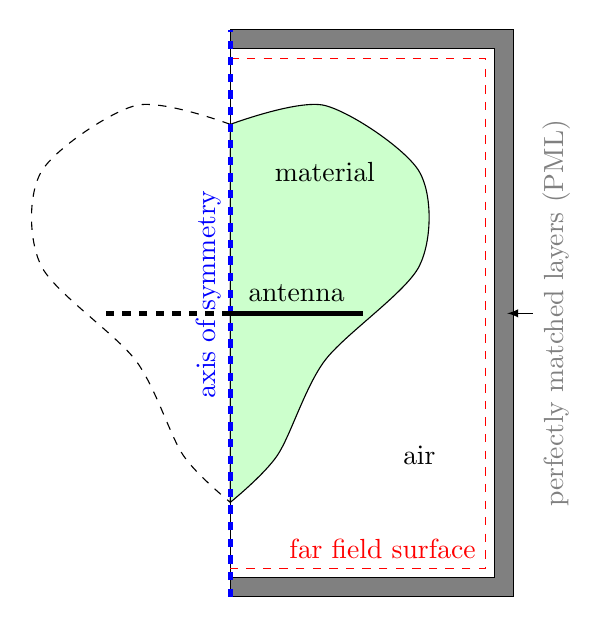
\begin{tikzpicture}[scale=1.2,>=latex]
      \draw[dashed] plot[smooth] coordinates {(0,2) (-1,2.2) (-2,1.5) (-2,0.5) (-1,-0.5) (-0.5,-1.5) (0,-2)} --cycle;
      \draw[fill=gray] (0,3) -- (3,3) -- (3,-3) -- (0,-3) -- cycle;
      \draw[fill=white] (0,2.8) -- (2.8,2.8) -- (2.8,-2.8) -- (0,-2.8) -- cycle;
      \draw[fill=green!20] plot[smooth] coordinates {(0,2) (1,2.2) (2,1.5) (2,0.5) (1,-0.5) (0.5,-1.5) (0,-2)} --cycle;
      \draw[dashed,red] (0,2.7) -- (2.7,2.7) -- (2.7,-2.7) -- (0,-2.7);
      \draw[dashed,blue,ultra thick] (0,-3) -- (0,3);
      \draw (2,-1.5) node {air};
      \draw (1,1.5) node {material};
      \draw[ultra thick] (0,0) -- (1.4,0) node[midway,above] {antenna};
      \draw[ultra thick,dashed] (0,0) -- (-1.4,0);
      \draw[red] (2.7,-2.7) node[anchor=south east] {far field surface};
      \draw[blue] (0,0.2) node[rotate=90,above] {axis of symmetry};
      \draw[->] (3.2,0) node[rotate=90,below,gray] {perfectly matched layers (PML)} -- (2.93,0);
%      \draw (1.5,3) node[above] {PEC};
    \end{tikzpicture}
  \end{center}
  \caption{Geometry of the finite element simulation. The material
    region has material parameters different than air, and the air
    region has $\epsilon_{\mrm{r}} = \mu_{\mrm{r}} = 1$. The antenna
    consists of a closed surface where one part is an aperture with a
    prescribed antenna field $\Ev_{\mrm{a}}$, and the other parts
    are PEC. The field on the far field surface is saved and
    postprocessed for each simulation. The simulation region (air and
    scatterer) $\Omega$ is surrounded by a region $\Omega_{\mrm{pml}}$
    of perfectly matched layers, having relative permittivity tensor
    $\epsm_{\mrm{r,pml}}$ and relative permeability tensor
    $\mum_{\mrm{r,pml}}$.}
  \label{fig:femgeom}
\end{figure}

The finite element method (FEM) formulation of the problem is based on
the weak formulation \eqref{eq:weakformulation2d}. The sought field is
expanded in basis functions as
$\Ev^{(m)}(\rv) = \sum_{n}E_{n}^{(m)}\Ev_{n}(\rv)$, and for each test
function $\vv(\rv)$, the equation \eqref{eq:weakformulation2d}
represents a row of a linear system of equations $Ax=b$ with $x$ as
the vector of unknowns $\{E_{1}^{(m)},E_{2}^{(m)},\ldots\}$ which can
be solved for. The process can be significantly automated with the use
of, for instance, the open source FEM project FEniCSx
\cite{Baratta+etal2023,Scroggs+etal2022a,Scroggs+etal2022b,Alnaes+etal2014},
where all necessary basis functions and infrastructure for mesh
handling, computing integrals and much more is already implemented. In
this paper, the finite element is chosen as a mixed element,
representing $(E_{\rho},E_{z})$ with curl conforming first kind
Nédélec (N1curl), and $E_{\varphi}$ with node based Lagrange (CG)
elements. The polynomial degree of the finite element can be chosen as
a parameter in FEniCSx.

In order to truncate \eqref{eq:equation2d} to a finite domain
$\Omega$, we surround the domain of interest with an absorbing
perfectly matched layer (PML) with complex and anisotropic material
parameters $\epsm_{\mrm{r,pml}}$ and $\mum_{\mrm{r,pml}}$ based on
stretched coordinates, see Figure~\ref{fig:femgeom} and
Appendix~\ref{app:pml} for explicit expressions of the material
parameters.

We include two different excitations: an antenna field $\Ev_{\mrm{a}}$
which is present only as tangential components on the aperture
$\Gamma_{\mrm{ant}}$ of an antenna, and a background field
$\Ev_{\mrm{b}}$ which corresponds to an incident wave propagating in a
background medium characterized by $\epsilon_{\mrm{r,b}}$ and
$\mu_{\mrm{r,b}}$. Typically, the background medium is considered to
be free space and we have
$\epsilon_{\mrm{r,b}} = \mu_{\mrm{r,b}} = 1$. We need to enforce
boundary conditions on the antenna surfaces, consisting of both
perfect electric conductor (PEC) parts, and an antenna aperture. On
the PEC surfaces $\Gamma_{\mrm{pec}}$, we require the boundary
condition $\nuv\times(\Ev^{(m)} + \Ev_{\mrm{b}}^{(m)}) = \Zv$, where
$\nuv$ is the surface normal and $\Ev^{(m)}+\Ev_{\mrm{b}}^{(m)}$
represents the total electric field. This is usually implemented as
Dirichlet boundary conditions, where the degrees of freedom
corresponding to the tangential electric fields are
prescribed. However, it can also be straight-forwardly implemented in
weak form by Nitsche's method \cite{Nitsche1971}. This uses the
functional
\begin{equation}
  \frac{\alpha}{h}\int_{\Gamma_{\mrm{pec}}} [\nuv\times(\Ev^{(m)} + \Ev_{\mrm{b}}^{(m)})] \cdot [\nuv\times\vv] \rho\diff\ell,
\end{equation}
where $h$ is the triangle diameter and $\alpha$ is a tuning parameter,
chosen as $\alpha=10$ in this work. On the antenna aperture
$\Gamma_{\mrm{ant}}$, we require the boundary condition
$\nuv\times(\Ev^{(m)}+\Ev_{\mrm{b}}^{(m)}-\Ev_{\mrm{a}}^{(m)})=\Zv$,
which can be implemented by the functional
\begin{equation}
  \frac{\alpha}{h}\int_{\Gamma_{\mrm{ant}}} [\nuv\times(\Ev^{(m)} + \Ev_{\mrm{b}}^{(m)} - \Ev_{\mrm{a}}^{(m)})] \cdot [\nuv\times\vv] \rho\diff\ell.
\end{equation}
This treats the antenna aperture surface as a metal boundary with
reflection coefficient $-1$ for the background field. The excitation
$\Ev_{\mrm{a}}$ for an antenna transmitting in a certain direction can
be approximated as the field values of a plane wave propagating in the
same direction evaluated on the antenna surface $\Gamma_{\mrm{ant}}$,
see Appendix~\ref{app:planewave}. In total, our finite element
formulation of the problem is then
\begin{multline}
  \iint_{\Omega} \left\{ - \mu_{\mrm{r}}^{-1}[\nabla_{m}\times\Ev^{(m)}]\cdot(\nabla_{m}\times\vv) + k^{2}\epsilon_{\mrm{r}} \Ev^{(m)}\cdot\vv \right\} \rho\diff\rho\diff z \\
  + \iint_{\Omega_{\mrm{pml}}} \left\{ -[\mum_{\mrm{r,pml}}^{-1}\cdot(\nabla_{m}\times\Ev^{(m)})]\cdot(\nabla_{m}\times\vv) + k^{2}[\epsm_{\mrm{r,pml}}\cdot\Ev^{(m)}]\cdot\vv \right\} \rho\diff\rho\diff z \\
  + \frac{\alpha}{h}\int_{\Gamma_{\mrm{pec}}} [\nuv\times(\Ev^{(m)} + \Ev_{\mrm{b}}^{(m)})] \cdot [\nuv\times\vv] \rho\diff\ell 
  + \frac{\alpha}{h}\int_{\Gamma_{\mrm{ant}}} [\nuv\times(\Ev^{(m)} + \Ev_{\mrm{b}}^{(m)} - \Ev_{\mrm{a}}^{(m)})] \cdot [\nuv\times\vv] \rho\diff\ell \\
  + \iint_{\Omega} k^{2}(\epsilon_{\mrm{r}} - \mu_{\mrm{r}}^{-1}\mu_{\mrm{r,b}}\epsilon_{\mrm{r,b}})\Ev_{\mrm{b}}^{(m)}\cdot\vv \rho\diff\rho\diff z
  = 0.
  \label{eq:femformulation}
\end{multline}
The last row is what remains after considering Maxwells' equations for
the total field $\Ev^{(m)}+\Ev_{\mrm{b}}^{(m)}$, and using that the
background field $\Ev_{\mrm{b}}^{(m)}$ satisfies the equation
$\iint_{\Omega}\mu_{\mrm{r,b}}^{-1}
(\nabla_{m}\times\Ev_{\mrm{b}}^{(m)}) \cdot (\nabla_{m}\times\vv)
\rho\diff\rho\diff z = \iint_{\Omega}
\epsilon_{\mrm{r,b}}k^{2}\Ev_{\mrm{b}}^{(m)}\cdot\vv
\rho\diff\rho\diff z$. Usually, only one of the excitations
$\Ev_{\mrm{a}}$ or $\Ev_{\mrm{b}}$ is nonzero.



\subsection{Symmetries}
\label{sec:symmetries}

Considering each polarization of an incident plane wave or antenna
excitation according to Appendix~\ref{app:planewave} and the general
relation $\BesselJ_{-n}(x) = (-1)^{n}\BesselJ_{n}(x)$, it is clear the
solution has the parities
\begin{align}
  &\hspace{-1cm}\text{$\theta$-polarization} && \hspace{-1cm}\text{$\phi$-polarization} \notag \\
  E_{\rho}^{(-m)} &= +E_{\rho}^{(m)} & E_{\rho}^{(-m)} &= -E_{\rho}^{(m)} \\
  E_{z}^{(-m)} &= +E_{z}^{(m)} & E_{z}^{(-m)} &= -E_{z}^{(m)} \\
  E_{\varphi}^{(-m)} &= -E_{\varphi}^{(m)} & E_{\varphi}^{(-m)} &= +E_{\varphi}^{(m)} 
\end{align}
Hence, for a fixed polarization it is sufficient to compute the
solution for $m\geq0$, and synthesize the solution in
postprocess. When polarizations are mixed, for instance one
polarization of an incident wave and another for the antenna
excitation, no symmetries can be used.


\section{Implementation in FEniCSx}
\label{sec:fenicsx}

The formulation \eqref{eq:femformulation} has been implemented in
FEniCSx, and is available at
\url{https://github.com/dsjoberg-git/rotsymsca}. The implementation is
largely inspired by the dolfinx demo \emph{Electromagnetic scattering
  from a sphere (asisymmetric)} at
\url{https://docs.fenicsproject.org/dolfinx/v0.9.0/python/demos/demo_axis.html}. The
key steps of the code are
\begin{itemize}
\item Create a mesh for the geometry using the Python interface to the
  open source mesh program Gmsh (\url{https://gmsh.info/})
  \cite{Geuzaine+Remacle2009}. At this stage, it is important to
  correctly label the geometry to identify regions with different
  materials and boundary conditions and pass this on to the main
  FEniCSx code.
\item Represent the three-dimensional electric field with a mixed
  finite element, where the in-plane field components
  $(E_{\rho},E_{z})$ are represented with Nédélec curl-conforming
  elements, and the out-of-plane field $E_{\phi}$ is represented with
  scalar node-based Lagrange elements. The polynomial degree of the
  finite elements can be chosen freely.
\item Set up material parameters and boundary conditions of the
  problem. This includes computing the PML material parameters using
  the expressions in Appendix~\ref{app:pml}.
\item Compute the solutions for each azimuth mode index $m$, and save
  relevant data for postprocessing.
\item Perform relevant postprocessing such as far field computation,
  near field plots, and projection on spherical vector harmonics.
\end{itemize}
Parallel processing using message passing interface (MPI) is mostly
transparent in FEniCSx, but requires attention in the postprocess
stage, where results from the different processes need to be gathered
in one single process. As of fall 2024, it is not possible to save the
solution when running in parallel (this is under current development
in FEniCSx), so only processed data is saved.

The code is provided as a main library \texttt{rotsymsca.py}, which
can be loaded in simulation scripts, see \texttt{verification.py} and
\verb+radome_simulations.py+ for examples. The mesh is generated in
\verb+mesh_rotsymradome.py+.



\section{Post processing}
\label{sec:postprocessing}

Since the field is computed for each azimuthal mode, some non-trivial
post processing is necessary to obtain the desired output data. This
data is primarily the far field amplitude, which can either be
computed directly or by first projecting the solution on the spherical
vector harmonics. For visualization purposes, we also need to consider
near field data.

\subsection{Far field computations}
\label{sec:farfield}

If the tangential electric and magnetic fields on a general surface
$S$ with outward normal $\nuv$ have been computed, the far field
amplitude in direction $\kuv$ is given by
\begin{equation}
  \Fv(\kuv) = \frac{\ju k}{4\pi} \kuv\times \iint_{S} \left[ \Ev(\rv)\times\nuv + \eta_{0}\kuv\times(\nuv\times\Hv(\rv)) \right] \eu^{\ju k\kuv\cdot\rv} \diff S.
\end{equation}
In the specific case of a rotationally symmetric structure, the
surface $S$ is described by a curve $\gamma$ in the $\rho$-$z$ plane,
and we have $\Fv(\kuv) = \sum_{m}\Fv^{(m)}(\kuv)$ where
\begin{equation}
  \Fv^{(m)}(\kuv) = \frac{\ju k}{4\pi} \kuv\times \int_{\vec{\rho}\in\gamma}\int_{\varphi=0}^{2\pi} \left[ \Ev^{(m)}(\rho,z)\times\nuv + \eta_{0}\kuv\times(\nuv\times\Hv^{(m)}(\rho,z)) \right] \eu^{\ju(k\kuv\cdot\rv-m\varphi)} \rho\diff\varphi\diff\ell
\end{equation}
The integral in the $\varphi$-direction is explicitly computed in
Appendix~\ref{app:farfield}, using the parameterization
$\kuv = \xuv\sin\theta\cos\phi + \yuv\sin\theta\sin\phi +
\zuv\cos\theta$, where $\theta$ is the polar angle and $\phi$ the
azimuth angle. Note that we distinguish between the far field
direction azimuth angle $\phi$ and the azimuth angle $\varphi$ used in
the cylindrical coordinate system where the vector components of the
electric field are defined. The result is
\begin{multline}
  \Fv^{(m)}(\theta,\phi) = \thetauv\frac{\ju k}{2}\ju^{m}\eu^{-\ju
    m\phi} \int_{\vec{\rho}\in\gamma} \Big\{ - \left[ C_{m}
    n_{z}E_{\varphi}^{(m)}
    - S_{m} (n_{\rho}E_{z}^{(m)} - n_{z}E_{\rho}^{(m)}) \right] \sin\phi \\
  + \left[ S_{m} n_{z}E_{\varphi}^{(m)}
    + C_{m} (n_{\rho}E_{z}^{(m)} - n_{z}E_{\rho}^{(m)}) \right] \cos\phi \\
  - \eta_{0} \left[ C_{m} n_{z}H_{\varphi}^{(m)}
    - S_{m} (n_{\rho}H_{z}^{(m)} - n_{z}H_{\rho}^{(m)}) \right] \cos\theta\cos\phi \\
  - \eta_{0}\left[ S_{m} n_{z}H_{\varphi}^{(m)}
    + C_{m} (n_{\rho}H_{z}^{(m)} - n_{z}H_{\rho}^{(m)}) \right] \cos\theta\sin\phi \\
  + \eta_{0} A_{m} n_{\rho}H_{\varphi}^{(m)}
  \sin\theta \Big\} \eu^{\ju kz\cos\theta} \rho\diff\ell \\
  + \phiuv \frac{\ju k}{2} \ju^{m}\eu^{-\ju
    m\phi}\int_{\vec{\rho}\in\gamma} \Big\{ - \left[ C_{m}
    n_{z}E_{\varphi}^{(m)}
    - S_{m} (n_{\rho}E_{z}^{(m)} - n_{z}E_{\rho}^{(m)}) \right] \cos\theta\cos\phi \\
  - \left[ S_{m} n_{z}E_{\varphi}^{(m)}
    + C_{m} (n_{\rho}E_{z}^{(m)} - n_{z}E_{\rho}^{(m)}) \right] \cos\theta\sin\phi \\
  + A_{m} n_{\rho}E_{\varphi}^{(m)} \sin\theta \\
  + \eta_{0} \left[ C_{m} n_{z}H_{\varphi}^{(m)}
    - S_{m} (n_{\rho}H_{z}^{(m)} - n_{z}H_{\rho}^{(m)}) \right] \sin\phi \\
  - \eta_{0}\left[ S_{m} n_{z}H_{\varphi}^{(m)} +
    C_{m} (n_{\rho}H_{z}^{(m)} -
    n_{z}H_{\rho}^{(m)}) \right] \cos\phi \Big\} \eu^{\ju kz\cos\theta}
  \rho\diff\ell
\end{multline}
where
\begin{align}
  A_{m} &= \BesselJ_{m}(k\rho\sin\theta) \\
  C_{m} &= \frac{1}{2}\left[ \eu^{\ju\phi}\BesselJ_{m-1}(k\rho\sin\theta) + \eu^{-\ju\phi}\BesselJ_{m+1}(k\rho\sin\theta) \right] \\
  S_{m} &= \frac{\ju}{2}\left[ \eu^{\ju\phi}\BesselJ_{m-1}(k\rho\sin\theta) - \eu^{-\ju\phi}\BesselJ_{m+1}(k\rho\sin\theta) \right]
\end{align}
This integral has been implemented in FEniCSx. It is important to
restrict the evaluations of the Bessel functions to cells adjacent to
the farfield boundary, in order to keep the overhead computations to a
minimum. 


\subsection{Projection on spherical vector harmonics}
\label{sec:sphericalvectorharmonics}

In order to limit the data needed to be saved from each simulation,
the far field results can be projected on spherical vector harmonics,
which also enables postprocessing of a three-dimensional radiation
pattern. We follow the definitions of spherical vector harmonics
presented in \cite{Hansen1988}, which is based on time convention
$\eu^{-\iu\omega t}$, whereas this document uses time convention
$\eu^{\ju\omega t}$. Define
\begin{equation}
  (\Ev_{smn}^{(c)},\Hv_{smn}^{(c)}) = \left(k\sqrt{\eta}\Fv_{smn}^{(c)}(r,\theta,\varphi), \frac{-\iu k}{\sqrt{\eta}}\Fv_{3-s,m,n}^{(c)}(r,\theta,\varphi)\right)
\end{equation}
where $\Fv_{smn}^{(c)}(r,\theta,\varphi)$ denotes the spherical vector
waves as defined in \cite{Hansen1988}, and
$\eta=\sqrt{\mu_{0}/\epsilon_{0}}$ is the wave impedance (note that
\cite{Hansen1988} uses the letter $\eta$ for the wave admittance, that
is, $\eta_{\mrm{Hansen}} = \sqrt{\epsilon_{0}/\mu_{0}}$). The outgoing
field is given by $c=3$ as
\begin{equation}
  (\Ev(\rv),\Hv(\rv)) = \sum_{smn}Q_{smn}^{(3)}(\Ev_{smn}^{(3)}(\rv),\Hv_{smn}^{(3)}(\rv)),
\end{equation}
where the expansion coefficients $Q_{smn}^{(3)}$ are determined from
the integral (where $\Ev$ and $\Hv$ are the electric and magnetic
field from the simulation, respectively)
\begin{equation}
  \iint_{S}\left\{\Ev\times\Hv_{s,-m,n}^{(1)} - \Ev_{s,-m,n}^{(1)}\times\Hv\right\} \cdot \nuv \diff S = (-1)^{m+1}Q_{smn}^{(3)}.
\end{equation}
The far field amplitude is
\begin{multline}
  \Fv(\theta,\varphi) = \lim_{r\rightarrow\infty}\frac{r}{\eu^{\iu kr}}\sum_{smn}Q_{smn}^{(3)}\Ev_{smn}^{(3)}(r,\theta,\varphi) = \lim_{r\rightarrow\infty} \frac{kr}{\eu^{\iu kr}}\sqrt{4\pi}\sqrt{\frac{\eta}{4\pi}} \sum_{smn}Q_{smn}^{(3)}\Fv_{smn}^{(3)}(r,\theta,\varphi) \\
  = \sqrt{\frac{\eta}{4\pi}}\sum_{smn}Q_{smn}^{(3)}\Kv_{smn}(\theta,\varphi),
  \label{eq:svwfarfield}
\end{multline}
where the functions $\Kv_{smn}(\theta,\varphi)$ are given in
\cite{Hansen1988}.  In order to use this procedure together with our
fields that have been computed using time convention
$\eu^{\ju\omega t}$, we first take the complex conjugate of our fields
$(\Ev,\Hv)$ that are recorded on a far field boundary. We then compute
the expansion coefficients $Q_{smn}^{(3)}$, and compute the far field
amplitude using \eqref{eq:svwfarfield}, and finally take the complex
conjugate of this result to obtain the expansion coefficients relevant
for the time convention $\eu^{\ju\omega t}$.

When only a cut of the far field amplitude is necessary, it is usually
faster to just compute the far field directly using the method in
Section~\ref{sec:farfield}. But when the far field should be evaluated
on the whole sphere, there is a clear benefit in first computing the
expansion coefficients $Q_{smn}^{(3)}$ which can subsequently be used
for any postprocessing of the far field.


\subsection{Near field plots}
\label{sec:nearfields}

For visualization purposes, it is necessary to compute the complex
amplitude of the near fields. We then need to compute the following
sum
\begin{equation}
  \Ev(\rv) = \sum_{m=-N}^{N}\Ev^{(m)}(\rv)\eu^{-\ju m\varphi}
  \label{eq:nearfield}
\end{equation}
for a fixed azimuth angle $\varphi$ (typically $\varphi=0$). Since
each azimuth mode is computed sequentially, we create a stored field
$\Ev(\rv)$ and add each mode sequentially according to
\eqref{eq:nearfield} until all modes have been computed. In order to
plot a full cross section, this means we need to compute the near
field not only for $\varphi=0$, but also for $\varphi=\pi$. Animations
of the near field can be created by plotting a sequence of 
$\Re\{\Ev(\rv)\eu^{\ju\omega t}\}$ for $\omega t\in[0,2\pi]$.



\section{Verification}
\label{sec:verification}

The code has been verified by computing the differential scattering
cross section for two spheres, one having radius $\lambda/2$ and the
other having radius $3\lambda$. We consider both PEC spheres and lossy
dielectric spheres, having relative permittivity $3(1-0.1\ju)$. The
degree of the finite elements is kept constant at 3, and the mesh size
is varied as $h/\lambda \in [0.4, 0.2, 0.1, 0.05, 0.025]$. The
farfield surface is at $\lambda/2$ from the sphere surface, the PML
starts at $\lambda/2$ from the farfield surface, and is $\lambda/2$
thick. The differential scattering cross section is computed for a
wave incident at $\theta=0$ and $\phi=0$, where it is sufficient to
use only modes $m=\pm1$ to represent the plane wave. The error is
computed using the results from miepython \cite{prahl_miepython_2025}
as reference value. The results for $E$-plane scattering are shown in
Figure~\ref{fig:hconvergence_Eplane}, and the $H$-plane results are in
Figure~\ref{fig:hconvergence_Hplane}.

It is seen that there is a clear convergence of the results with
decreasing mesh size for all considered cases.

\begin{figure}
  \begin{center}
    \begin{tabular}{cc}
      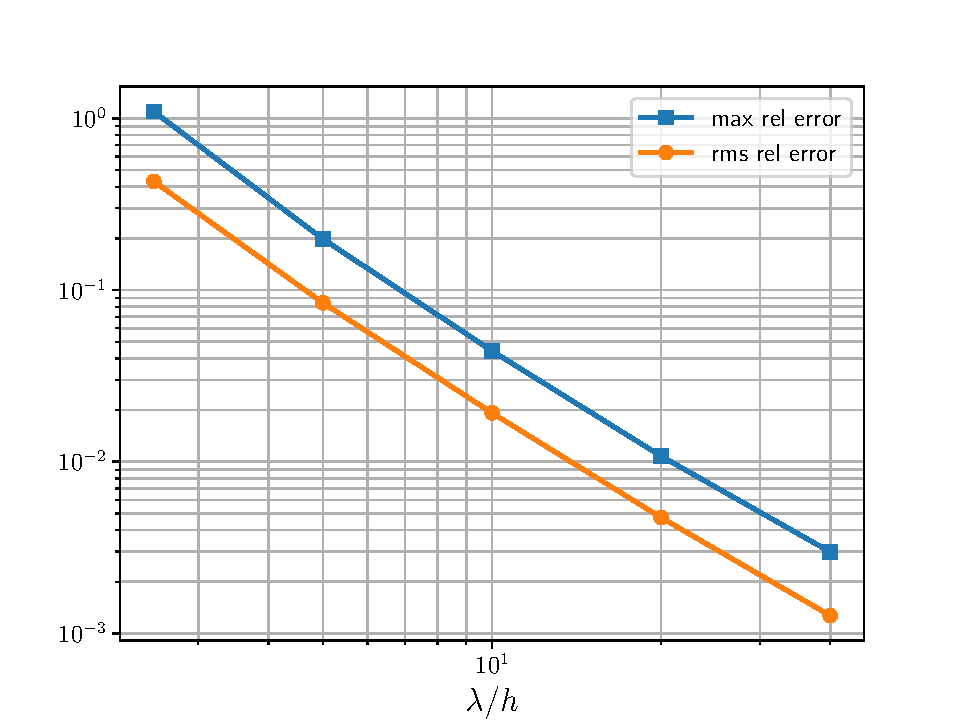
\includegraphics[width=0.45\textwidth]{verification_0.5lambda_pec_theta} &
      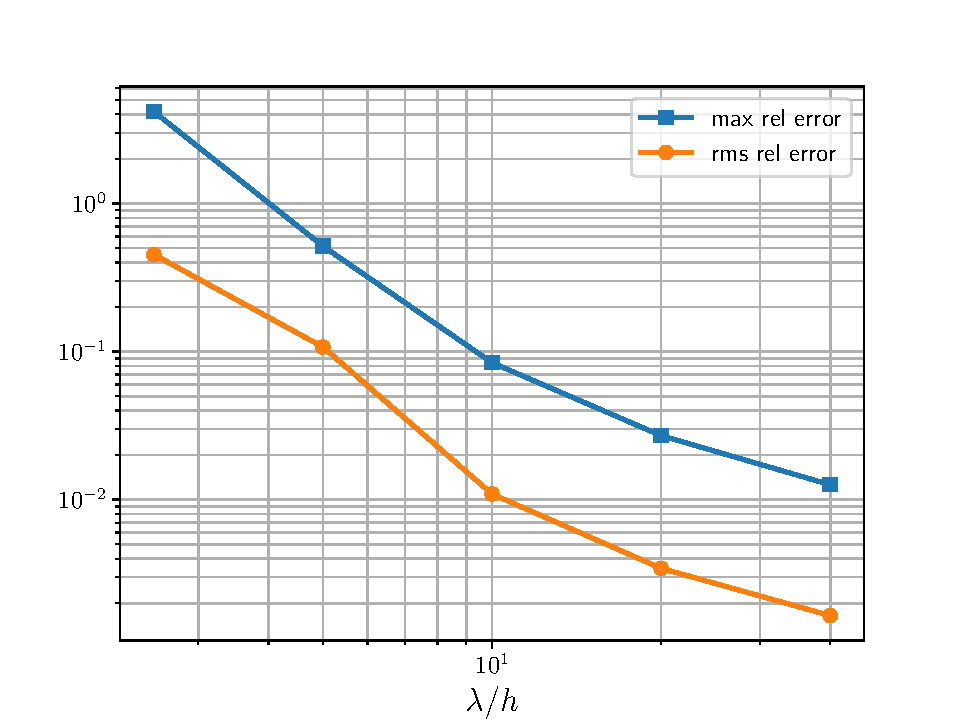
\includegraphics[width=0.45\textwidth]{verification_3.0lambda_pec_theta} \\
      (a) & (b) \\
      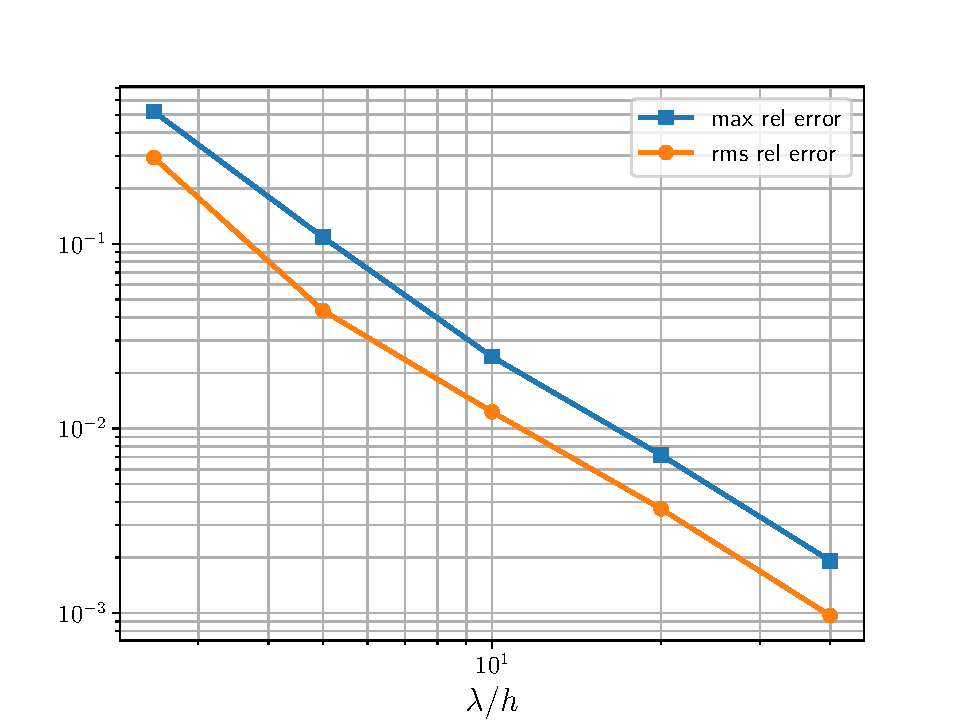
\includegraphics[width=0.45\textwidth]{verification_0.5lambda_dielectric_theta} &
      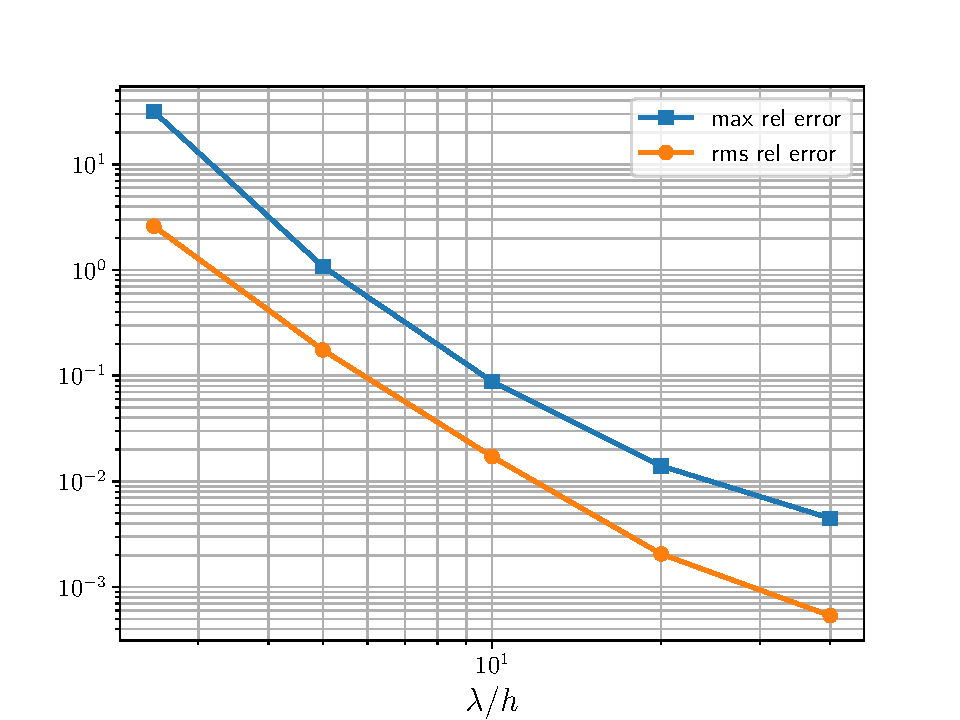
\includegraphics[width=0.45\textwidth]{verification_3.0lambda_dielectric_theta} \\
      (c) & (d) 
    \end{tabular}
  \end{center}
  \caption{Results for $h$-convergence of $E$-plane differential
    scattering cross section of some spheres. (a) PEC sphere radius
    $\lambda/2$, (b) PEC sphere radius $3\lambda$, (c) lossy
    dielectric sphere radius $\lambda/2$, (d) lossy dielectric sphere
    radius $3\lambda$.}
  \label{fig:hconvergence_Eplane}
\end{figure}

\begin{figure}
  \begin{center}
    \begin{tabular}{cc}
      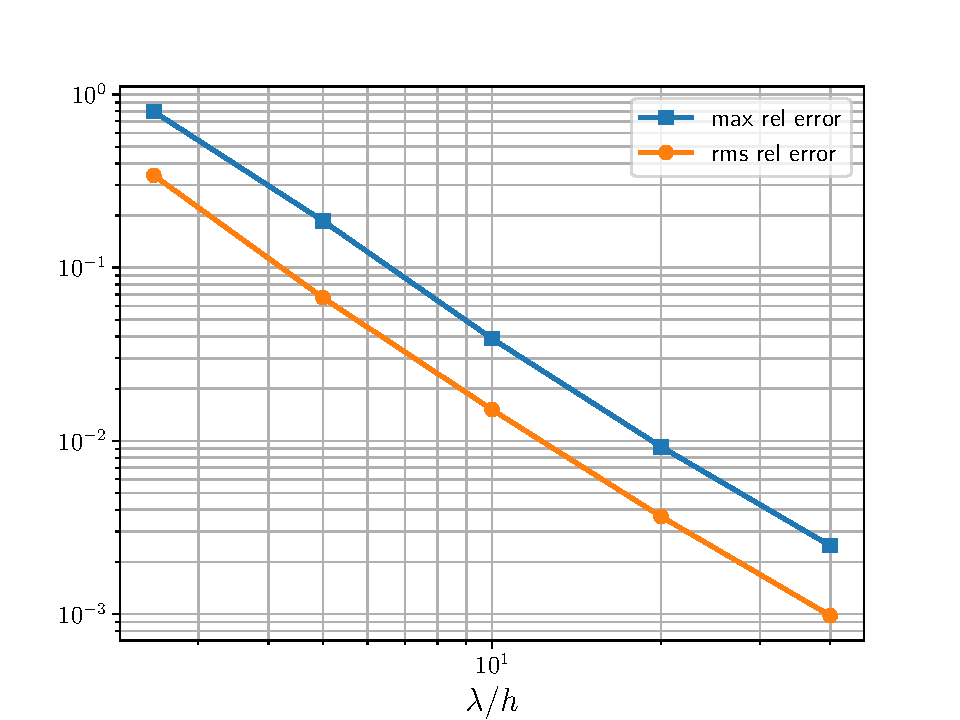
\includegraphics[width=0.45\textwidth]{verification_0.5lambda_pec_phi} &
      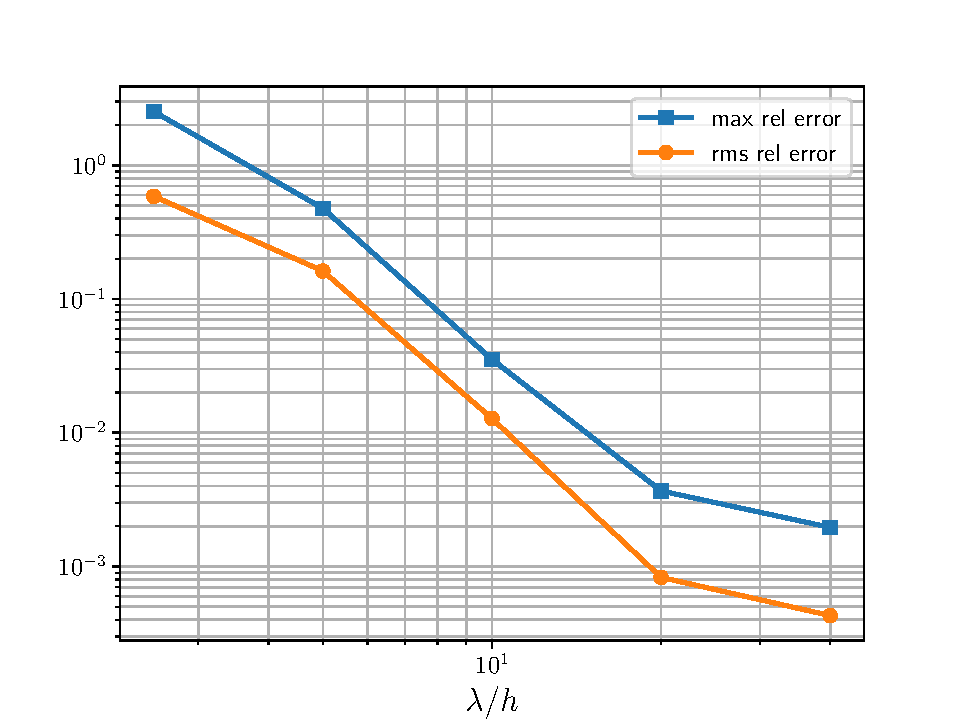
\includegraphics[width=0.45\textwidth]{verification_3.0lambda_pec_phi} \\
      (a) & (b) \\
      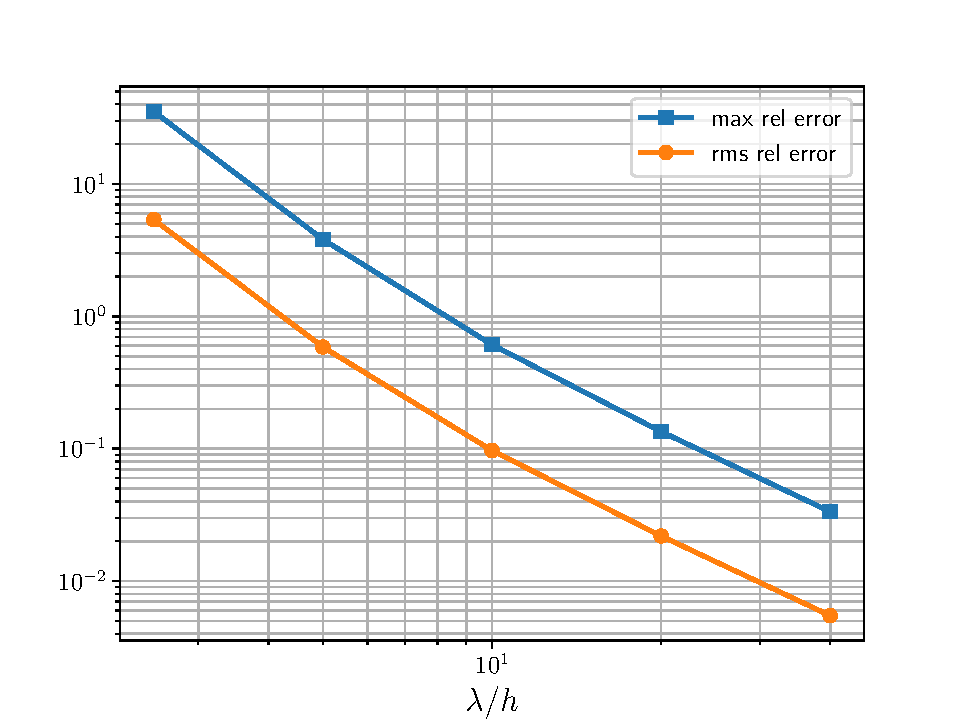
\includegraphics[width=0.45\textwidth]{verification_0.5lambda_dielectric_phi} &
      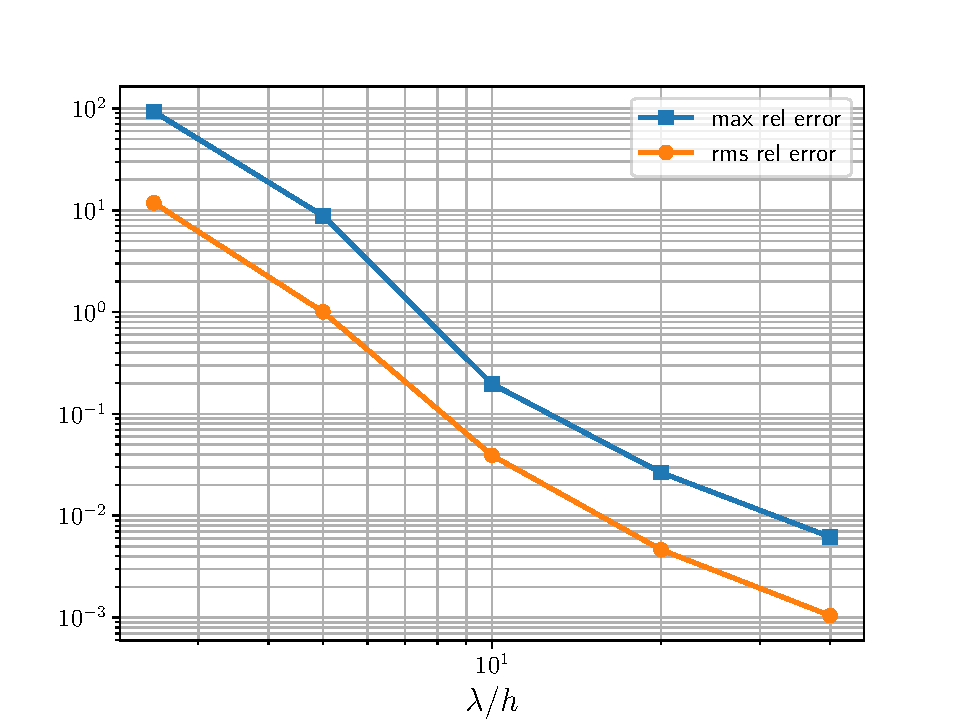
\includegraphics[width=0.45\textwidth]{verification_3.0lambda_dielectric_phi} \\
      (c) & (d) 
    \end{tabular}
  \end{center}
  \caption{Results for $h$-convergence of $H$-plane differential
    scattering cross section of some spheres. (a) PEC sphere radius
    $\lambda/2$, (b) PEC sphere radius $3\lambda$, (c) lossy
    dielectric sphere radius $\lambda/2$, (d) lossy dielectric sphere
    radius $3\lambda$.}
  \label{fig:hconvergence_Hplane}
\end{figure}

\section{Application to a radome geometry}

\begin{figure}
  \begin{center}
    \begin{tikzpicture}[>=latex]
      \pgfmathsetmacro{\ogivefactor}{2}
      \pgfmathsetmacro{\lda}{0.5}
      \pgfmathsetmacro{\w}{10*\lda}
      \pgfmathsetmacro{\H}{5*\lda}
      \pgfmathsetmacro{\epsr}{3}
      \pgfmathsetmacro{\d}{\lda/2/sqrt(\epsr)}
      \pgfmathsetmacro{\da}{\lda/2}
      \pgfmathsetmacro{\Rb}{\w/2 + \da + \d}
      \pgfmathsetmacro{\Lb}{\Rb*\ogivefactor}
      \pgfmathsetmacro{\rb}{(\Rb^2 + \Lb^2)/(2*\Rb)}
      \pgfmathsetmacro{\Ra}{\Rb - \d}
      \pgfmathsetmacro{\ra}{\rb - \d}
      \pgfmathsetmacro{\La}{sqrt(\ra^2 - (\rb - \Rb)^2)}
      \draw[smooth, samples=100, domain=0:1.0001] plot({sqrt(\ra^2-(\La*\x)^2) + \Ra - \ra}, \La*\x);
      \draw[smooth, samples=100, domain=0:1.0001] plot({sqrt(\rb^2-(\Lb*\x)^2) + \Rb - \rb}, \Lb*\x);
      \draw[smooth, samples=100, domain=0:1.001] plot({-(sqrt(\ra^2-(\La*\x)^2) + \Ra - \ra)}, \La*\x);
      \draw[smooth, samples=100, domain=0:1.001] plot({-(sqrt(\rb^2-(\Lb*\x)^2) + \Rb - \rb)}, \Lb*\x);
      \draw (\Ra,0) -- (\Ra,-\H) -- (\Rb,-\H) -- (\Rb,0);
      \draw (-\Ra,0) -- (-\Ra,-\H) -- (-\Rb,-\H) -- (-\Rb,0);
      \draw[ultra thick] (-\w/2,0) -- (\w/2,0);

      \draw[<->, shift={(0,-0.4)}] (-\w/2,0) -- (\w/2,0) node[midway, below] {$w$};
      \draw[<->, shift={(0,-1.4)}] (-\Ra,0) -- (\Ra,0) node[midway, below] {$2R_{\mrm{a}}$};
      \draw[<->, shift={(0,-2.4)}] (-\Rb,0) -- (\Rb,0) node[midway, below] {$2R_{\mrm{b}}$};
      \draw[<->, shift={(-0.5,0)}] (-\Rb,0) -- (-\Rb,-\H) node[midway,left] {$H$};
      \draw[<->] (0,0) -- (0,\La) node[midway, right] {$L_{\mrm{a}}$};
      \draw[<->, shift={(-\Rb-0.5,0)}] (0,0) -- (0,\Lb) node[midway, left] {$L_{\mrm{b}}$};
      \draw[dashed] (-\Rb-1,\Lb) -- (0.5,\Lb);
      \draw[->] (\Ra-0.5,-1) -- (\Ra,-1);
      \draw[->] (\Rb+1,-1) -- (\Rb,-1) node[midway,above] {$d$};
      \draw[->] (3,4) node[right] {$x=\sqrt{\rho_{\mrm{b}}^{2}-z^{2}} + R_{\mrm{b}} - \rho_{\mrm{b}}$} -- ({sqrt(\rb^2-(0.6*\Lb)^2)+\Rb-\rb},0.6*\Lb);
      \draw[->] (3,2) node[right] {$x=\sqrt{\rho_{\mrm{a}}^{2}-z^{2}} + R_{\mrm{a}} - \rho_{\mrm{a}}$} -- ({sqrt(\ra^2-(0.3*\La)^2)+\Ra-\ra},0.3*\La);
      \draw[->] (\Rb+0.5,0) -- (\Rb+1.5,0) node[right] {$x$};
      \draw[->] (0,\Lb+0.5) -- (0,\Lb+1.5) node[above] {$z$};
    \end{tikzpicture}
  \end{center}
  \caption{Geometry parameters of the ogive radome, adapted from
    \url{https://en.wikipedia.org/wiki/Nose_cone_design}. The radius
    of curvature for the ogive parts is computed from the other
    parameters as
    $\rho_{\mrm{a,b}} = (R_{\mrm{a,b}}^{2} +
    L_{\mrm{a,b}}^{2})/(2R_{\mrm{a,b}})$, and the thickness of the
    radome at the base is $d = R_{\mrm{b}} - R_{\mrm{a}}$. The antenna
    width is $w$, and the distance between the antenna and the radome
    is $d_{0} = R_{\mrm{a}} - w/2$.}
  \label{fig:ogiveradome_geometry}
\end{figure}

We analyze an ogive-shaped radome, which is a common design for a nose
cone radome, see Figure~\ref{fig:ogiveradome_geometry}. This design
has several features of a realistic radome, in particular a pointed
tip. The baseline parameters of the radome, corresponding to
Figure~\ref{fig:ogiveradome_geometry}, are chosen as
\begin{itemize}
\item $f_{0} = 10\unit{GHz}$ (frequency)
\item $\lambda_{0} = \cu/f_{0}$ (wavelength)
\item $w = 10\lambda_{0} = 0.300\unit{m}$ (diameter of antenna)
\item $d_{0} = \lambda_{0}/2 = 0.0150\unit{m}$ (distance from antenna to radome)
\item $\epsilon_{\mrm{r}} = 3$ (relative permittivity of radome, lossless)
\item $d = \lambda_{0}/(2\sqrt{\epsilon_{\mrm{r}}}) = 8.7\unit{mm}$
  (thickness of radome)
\item $\alpha = 2$ (ogive shape factor)
\item $R_{\mrm{a}} = w/2 + d_{0} = 0.165\unit{m}$
\item $L_{\mrm{a}} = \alpha R_{\mrm{a}} = 0.330\unit{m}$
\item $\rho_{\mrm{a}} = (R_{\mrm{a}}^{2} + L_{\mrm{a}}^{2})/(2R_{\mrm{a}}) = 0.412\unit{m}$
\item $R_{\mrm{b}} = w/2 + d_{0} + d = 0.174\unit{m}$
\item $L_{\mrm{b}} = \alpha R_{\mrm{b}} = 0.347\unit{m}$
\item $\rho_{\mrm{b}} = (R_{\mrm{b}}^{2} + L_{\mrm{b}}^{2})/(2R_{\mrm{b}}) = 0.434\unit{m}$
\item $H = 5\lambda_{0} = 0.150\unit{m}$
\end{itemize}
The antenna is implemented as a circular antenna with thickness
$0.1\lambda_{0}$ and a cosine-tapering in the radial direction, that
is, the antenna field is
\begin{equation}
  \Ev_{\mrm{a}}(\rv) = \Ev_{0}\eu^{-\ju\kv\cdot\rv}\cos(\pi\rho/w), \quad \rv\in\Gamma_{\mrm{ant}}
\end{equation}
where the expression for a plane wave in \eqref{eq:planewave} is used
to express $\Ev_{0}\eu^{-\ju\kv\cdot\rv}$ in azimuthal modes. The
baseline antenna is ten wavelengths in diameter, making the radiation
highly directive.

The excitation corresponding to an incident plane wave is
$\Ev_{\mrm{b}}(\rv) = \Ev_{0}\eu^{-\ju\kv\cdot\rv}$. In both the antenna
excitation and the plane wave excitation, the azimuth modes are found
from the expressions in Appendix~\ref{app:planewave}.


\subsection{Parameter variations}

From the baseline geometry we make a number of parameter variations in
the simulations:
\begin{itemize}
\item Electric field in $\theta$ (TM, in plane) or $\phi$ (TE, out of
  plane) polarization.
\item Angle of incidence $\theta\in[0^{\circ},10^{\circ},20^{\circ},30^{\circ},40^{\circ},50^{\circ}]$.
\item With and without radome.
\item Either with a transmitting antenna or scattering from an
  incident plane wave.
\item Antenna width
  $w\in[10\lambda_{0},20\lambda_{0},30\lambda_{0}]$. Note that the
  radome thickness is $\lambda_{0}/(2\sqrt{\epsilon_{\mrm{r}}})$ in
  all cases, that is, the radome is always transparent.
\end{itemize}
All combinations of these parameters have been run, and the results
are discussed in the following subsection. The mesh size was chosen as
$h=\lambda_{0}/10$, and the structure was surrounded by a cylindrical
PML with thickness $\lambda_{0}/2$ at distance $\lambda_{0}$ from the
radome in all directions.

\subsection{Results}
\label{sec:results}

Typical examples of near field plots are given in
Figure~\ref{fig:nearfields}, where the scattered field is plotted for
a plane wave excitation, and the total field is plotted for a
transmitting antenna excitation. The results are given for three
different radome sizes, corresponding to antenna widths
$w=10\lambda_{0},20\lambda_{0},30\lambda_{0}$, using
$\phi$-polarization.

For the incident plane wave (top row), it is seen there is a
significant scattered field inside the radome cavity; this is due to
the delay through the radome wall, and does not necessarily mean the
radome scatters in the monostatic direction. There is also a strong
scattered field in the region beneath the antenna, which is necessary
to cancel the incident field in this shadow region. Some significant
scattering is observed near the pointed tip of the radome, especially
for the larger radome.

For the transmitting case, we can clearly see a reflection lobe
travelling to the left. This is due to imperfect transmission of the
wave through the radome wall, which was designed with normal incidence
in mind. The curvature of the radome further shapes this reflection lobe.

\newlength{\myfigwidth}
\setlength{\myfigwidth}{0.5\linewidth}

\begin{figure}
  \begin{center}
    \begin{tabular}{ccc}
      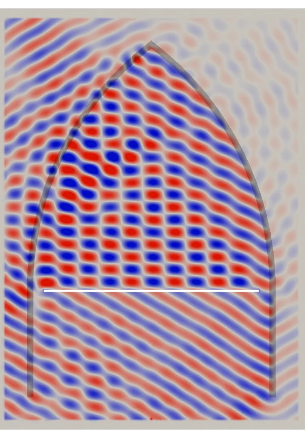
\includegraphics[width=0.3\linewidth]{nearfield_scattering_theta30_w10} &
      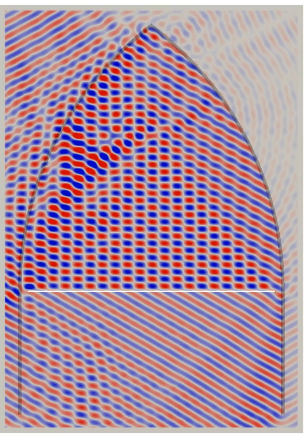
\includegraphics[width=0.3\linewidth]{nearfield_scattering_theta30_w20} &
      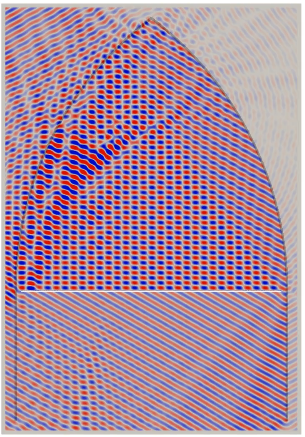
\includegraphics[width=0.3\linewidth]{nearfield_scattering_theta30_w30} \\
      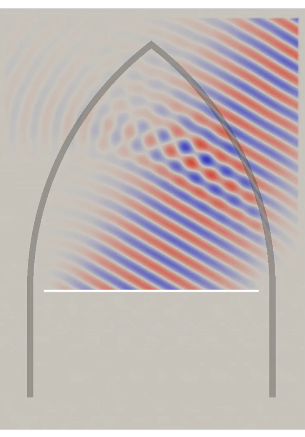
\includegraphics[width=0.3\linewidth]{nearfield_transmitting_theta30_w10} &
      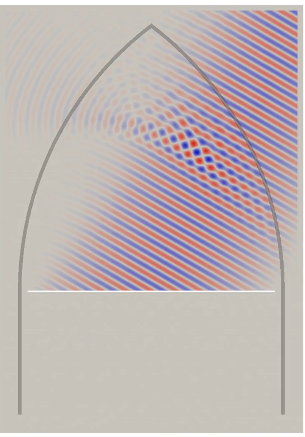
\includegraphics[width=0.3\linewidth]{nearfield_transmitting_theta30_w20} &
      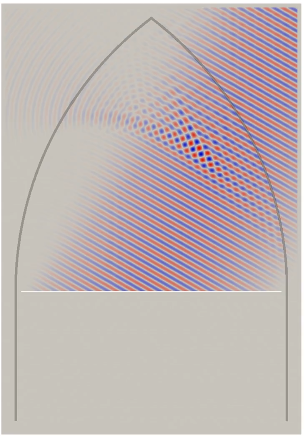
\includegraphics[width=0.3\linewidth]{nearfield_transmitting_theta30_w30} 
    \end{tabular}
  \end{center}
  \caption{Near field plots of scattered field when subjected to an
    incident plane wave from $\theta=30^{\circ}$ (top row) and total
    field with transmitting antenna towards $\theta=30^{\circ}$
    (bottom row) from antenna with radome present, antenna widths
    $w=10\lambda_{0},20\lambda_{0},30\lambda_{0}$ (from left to
    right).}
  \label{fig:nearfields}
\end{figure}

Far field results in the plane of incidence for an incident plane wave
are shown in Figure~\ref{fig:scatteringw10} for antenna width
$w=10\lambda_{0}$. Both polarizations and the cases with and without
radome are reported. It is seen that there is a significantly
increased bistatic scattering at some angles for the
$\phi$-polarization when the radome is present, whereas the
corresponding effect is smaller for the $\theta$-polarization.

\begin{figure}
  \begin{center}
    \begin{tabular}{cc}
      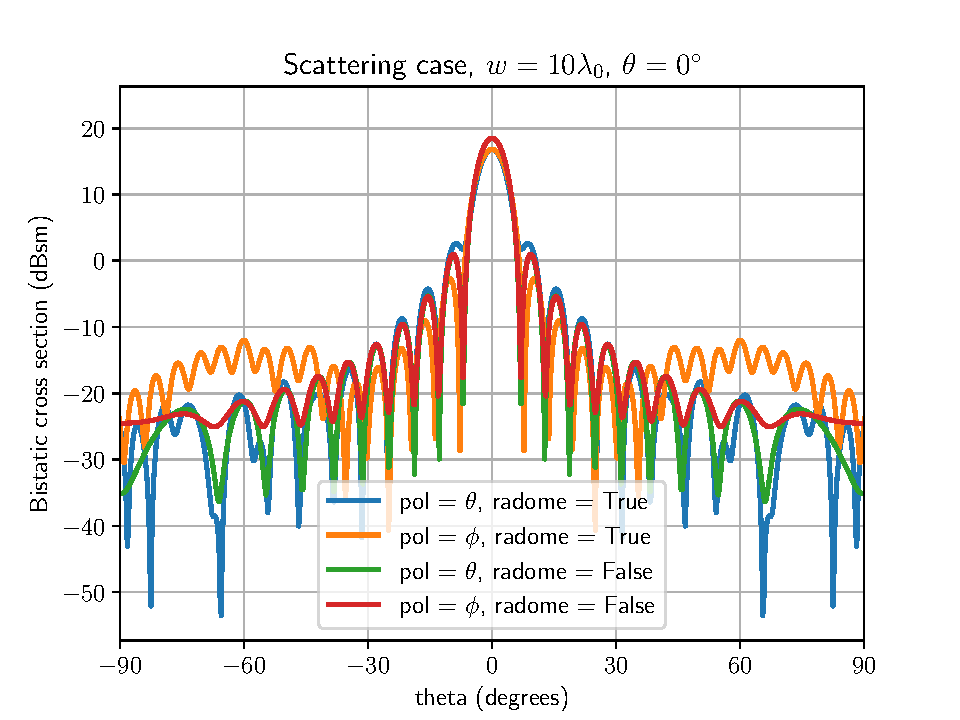
\includegraphics[width=\myfigwidth]{scattering_w10_theta0} &
      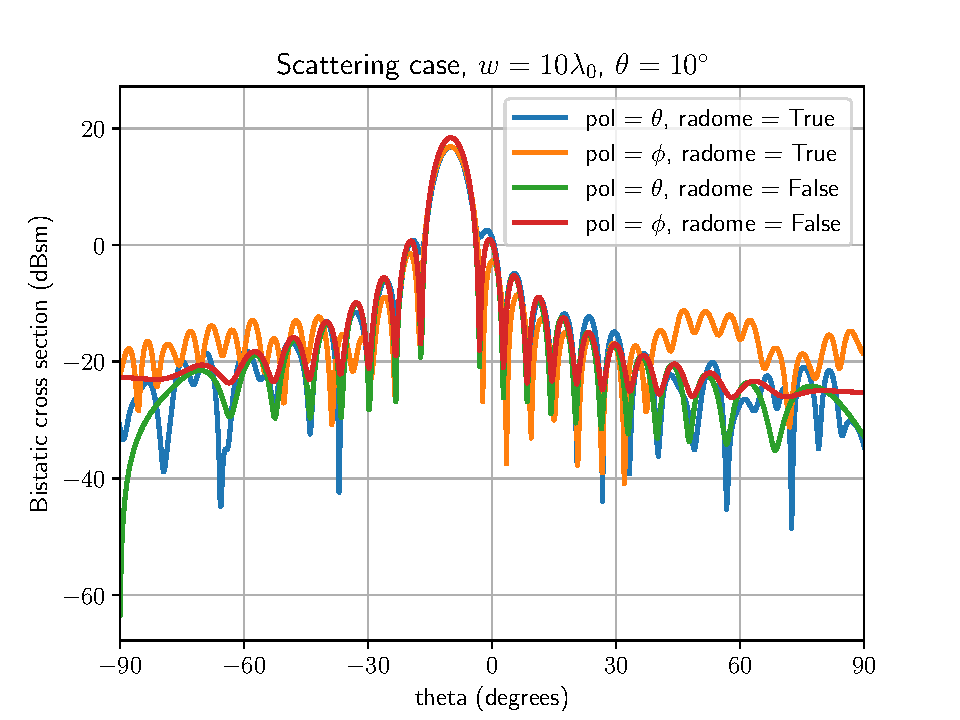
\includegraphics[width=\myfigwidth]{scattering_w10_theta10} \\
      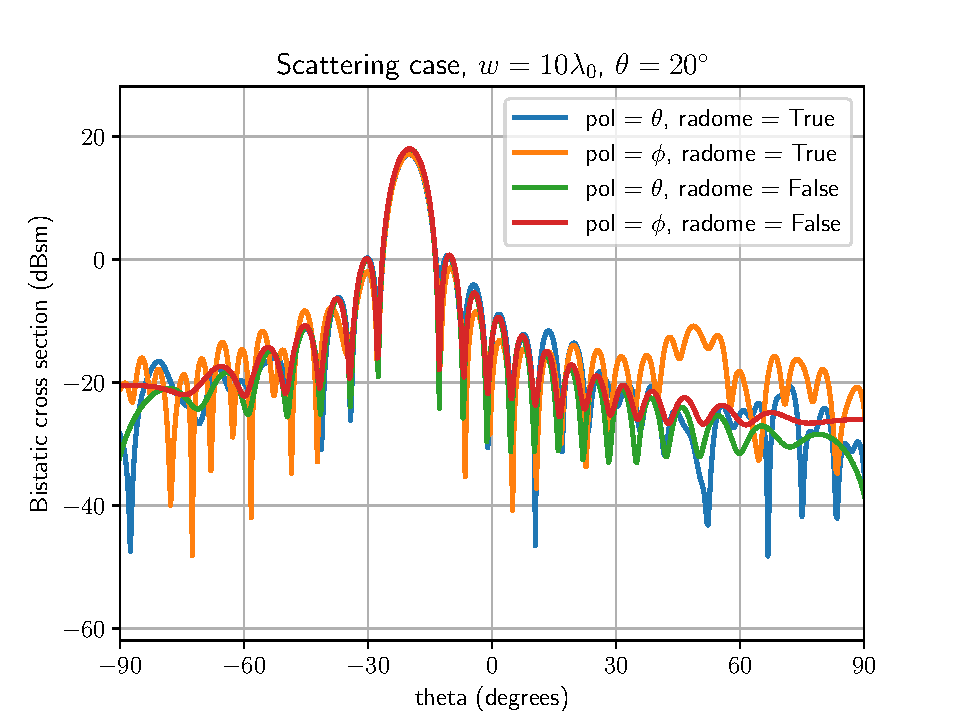
\includegraphics[width=\myfigwidth]{scattering_w10_theta20} &
      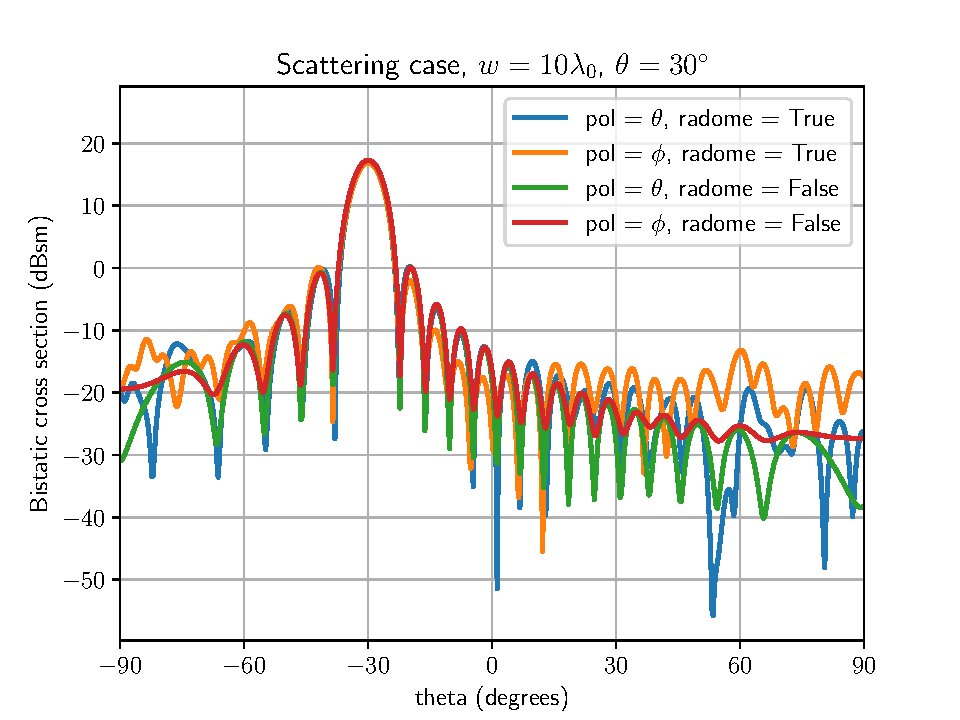
\includegraphics[width=\myfigwidth]{scattering_w10_theta30} \\
      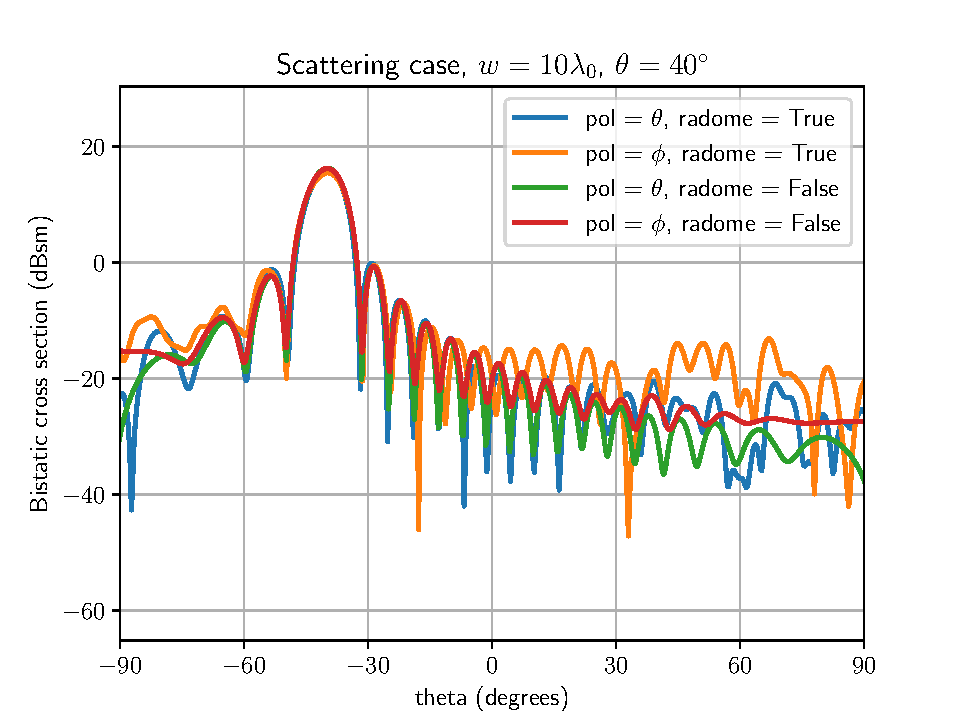
\includegraphics[width=\myfigwidth]{scattering_w10_theta40} &
      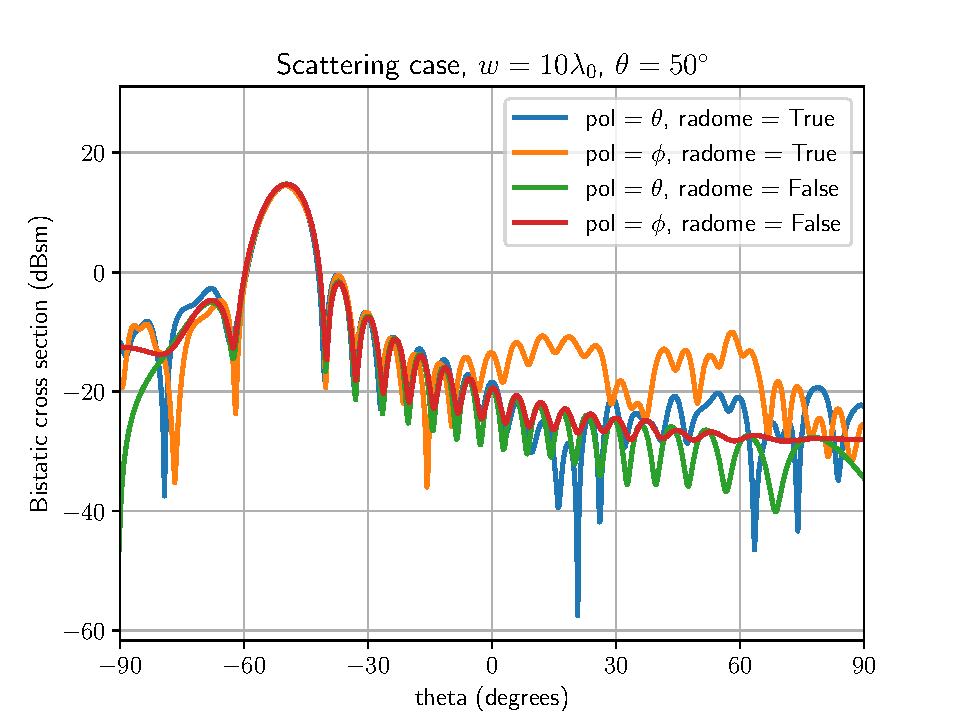
\includegraphics[width=\myfigwidth]{scattering_w10_theta50} 
    \end{tabular}
  \end{center}
  \caption{Scattering from antenna with and without radome, antenna
    width $w=10\lambda_{0}$.}
  \label{fig:scatteringw10}
\end{figure}

In Figure~\ref{fig:transmissionw10}, the corresponding results are
plotted for the transmitting antenna excitation. Here, we observe
significantly increased and broad side lobe levels with the radome
present, for both polarizations. This is the reflection lobe earlier
observed in the near field plots in Figure~\ref{fig:nearfields}, due
to imperfect transmission through the radome wall. A somewhat
increased side lobe around $-40^{\circ}$ can be observed in the
$\phi$-polarization without radome for high steering angles, in
particular $\theta=40^{\circ}$. This indicates there is some
scattering occurring at the edges of the antenna for this
polarization, even without the radome present.


\begin{figure}
  \begin{center}
    \begin{tabular}{cc}
      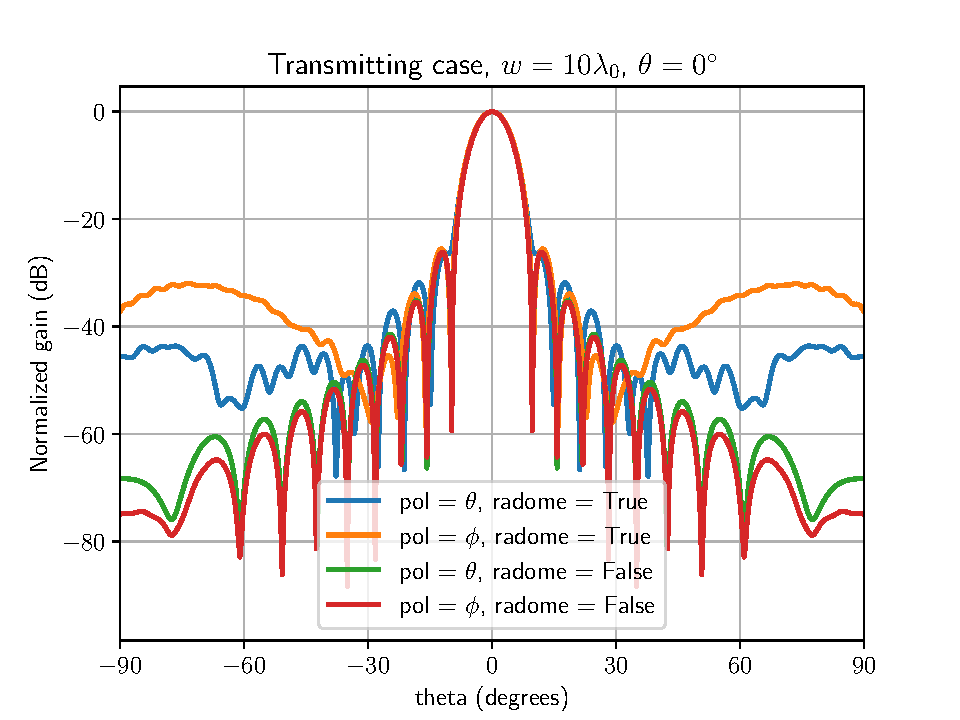
\includegraphics[width=\myfigwidth]{transmitting_w10_theta0} &
      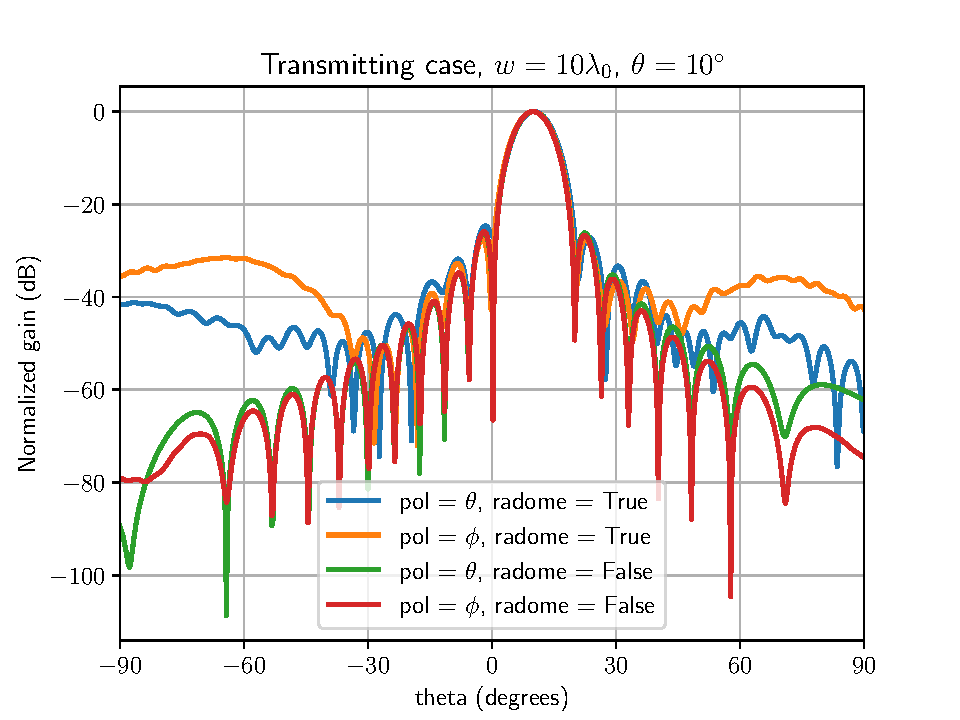
\includegraphics[width=\myfigwidth]{transmitting_w10_theta10} \\
      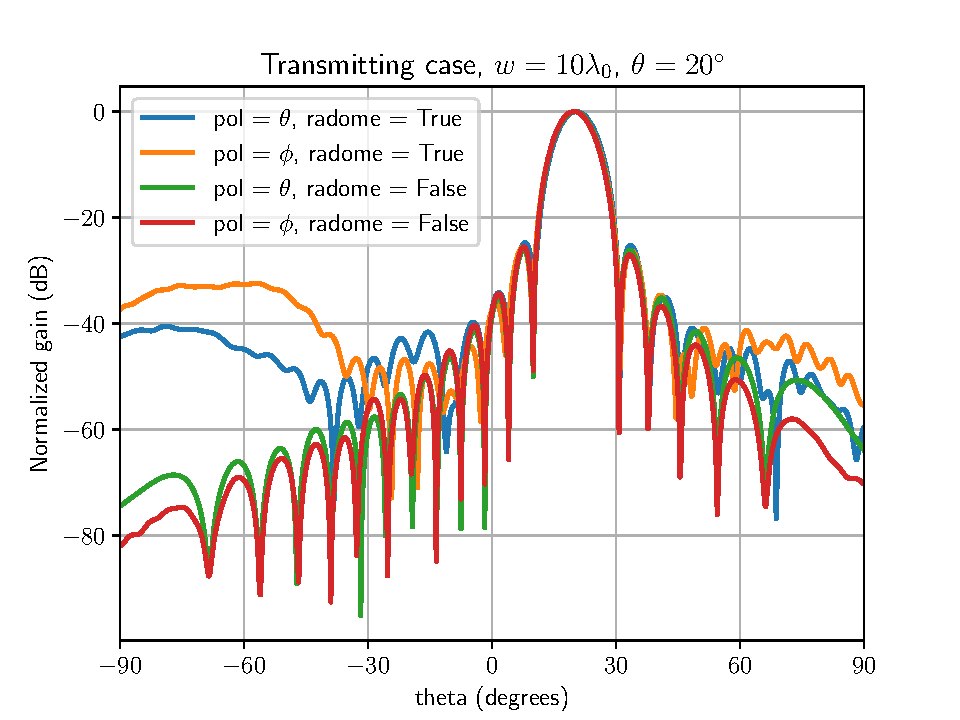
\includegraphics[width=\myfigwidth]{transmitting_w10_theta20} &
      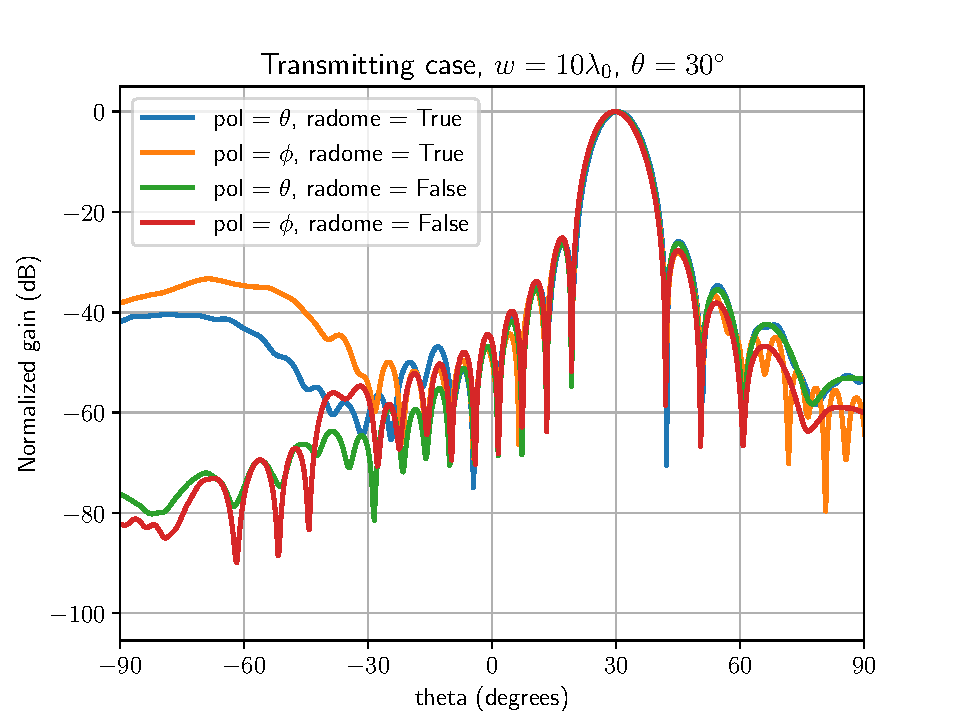
\includegraphics[width=\myfigwidth]{transmitting_w10_theta30} \\
      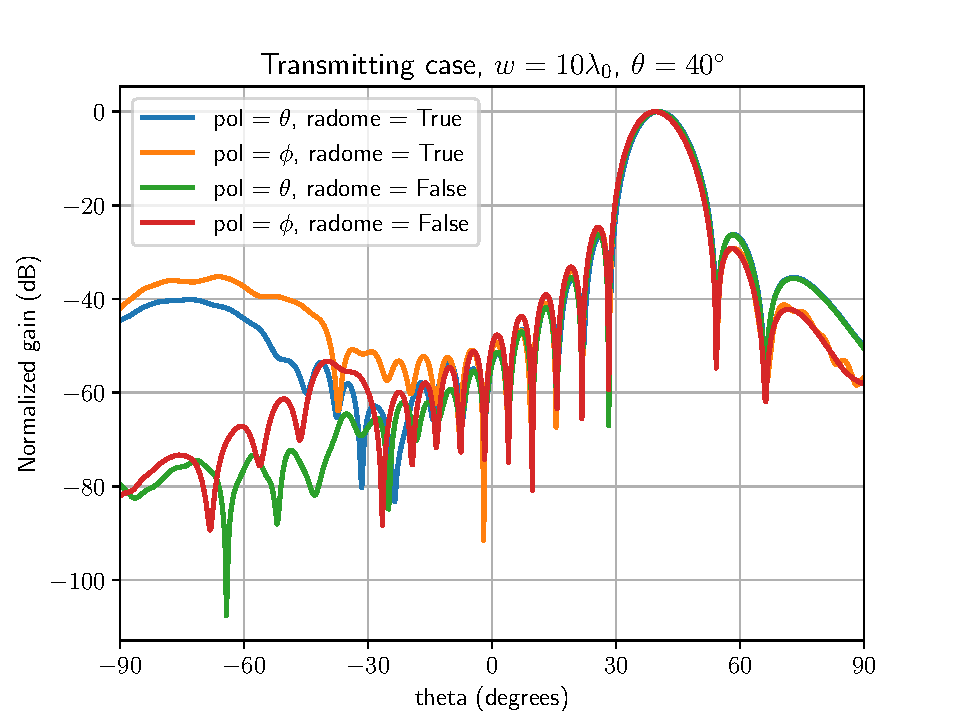
\includegraphics[width=\myfigwidth]{transmitting_w10_theta40} &
      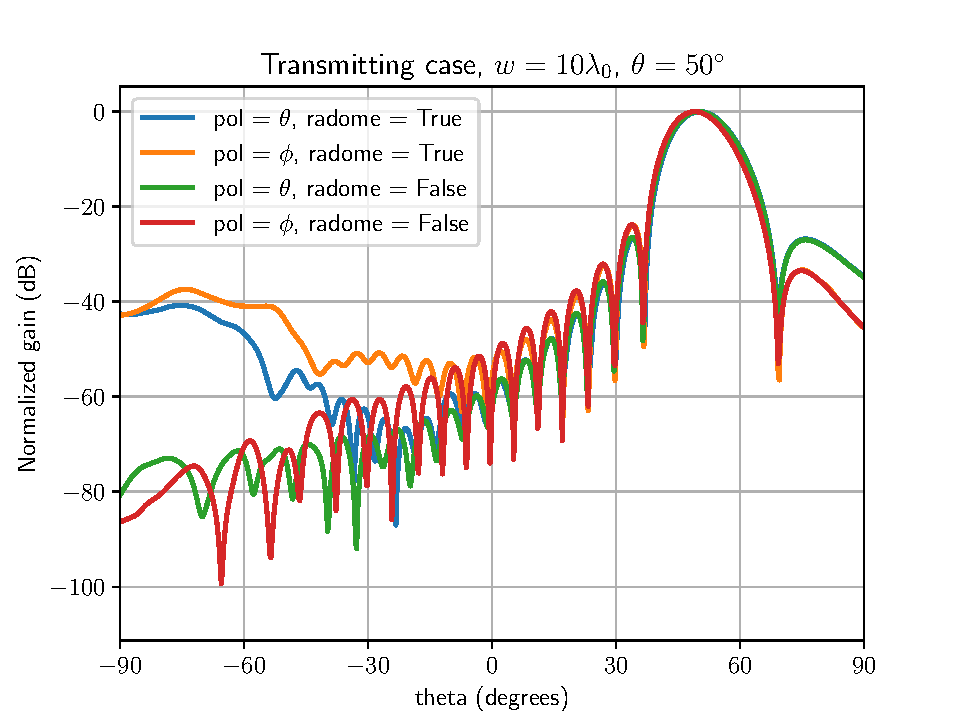
\includegraphics[width=\myfigwidth]{transmitting_w10_theta50} 
    \end{tabular}
  \end{center}
  \caption{Transmission from antenna with and without radome, antenna
    width $w=10\lambda_{0}$.}
  \label{fig:transmissionw10}
\end{figure}

Figures~\ref{fig:scatteringw20} and \ref{fig:scatteringw30} show the
same results as Figure~\ref{fig:scatteringw10} but for antenna widths
$w=20\lambda_{0}$ and $30\lambda_{0}$, respectively. It is seen that
the trend of increased side lobes for the $\phi$-polarization is
maintained for the larger radome sizes, with a more moderate increase
for the $\theta$-polarization.

\begin{figure}
  \begin{center}
    \begin{tabular}{cc}
      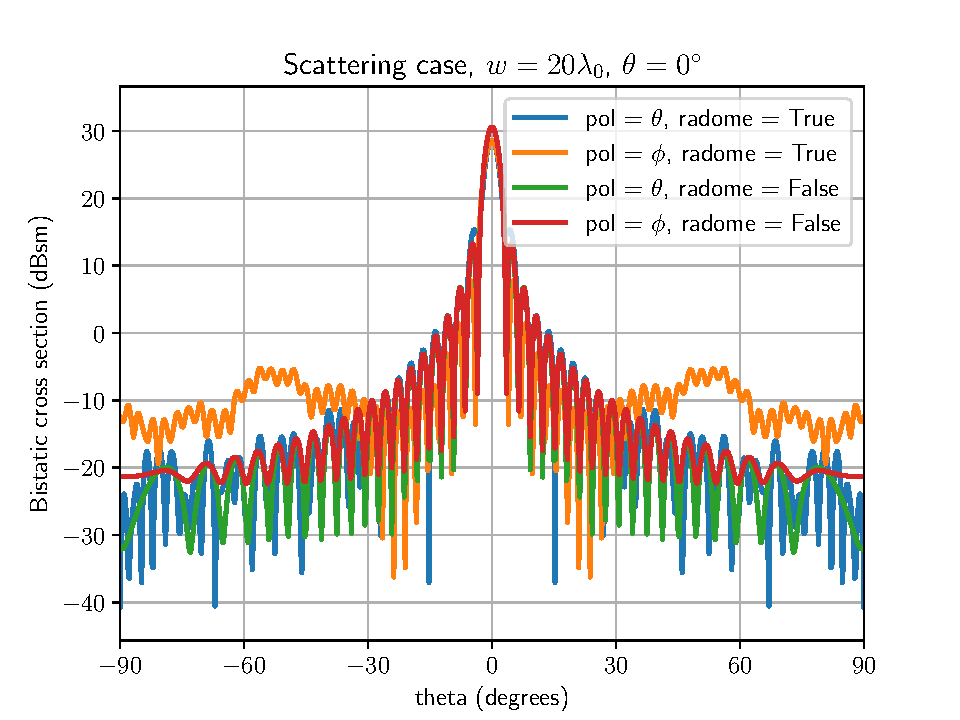
\includegraphics[width=\myfigwidth]{scattering_w20_theta0} &
      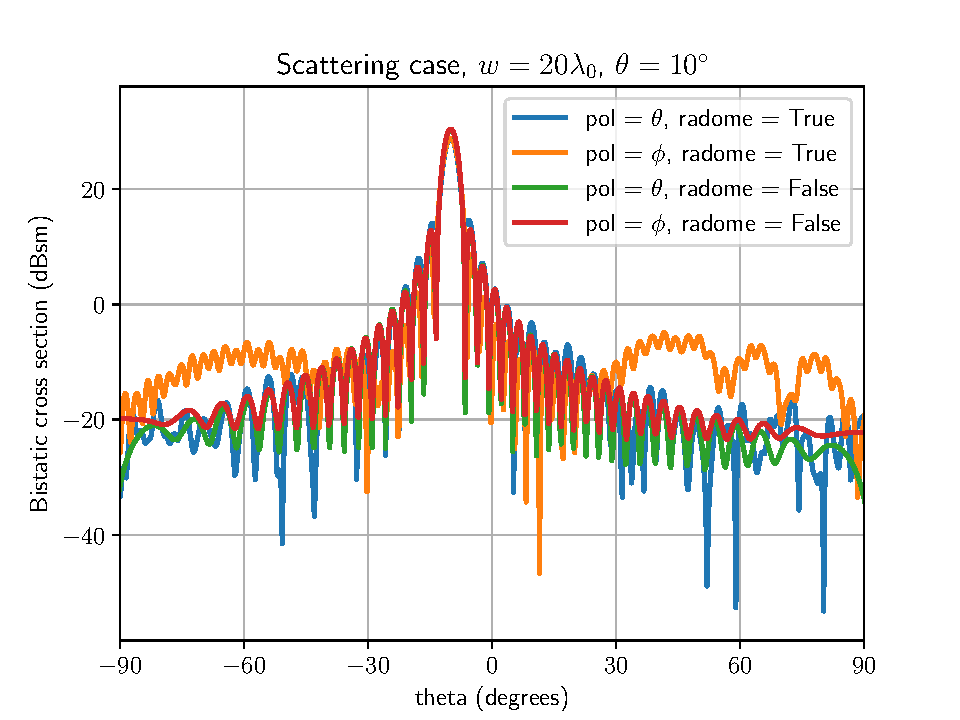
\includegraphics[width=\myfigwidth]{scattering_w20_theta10} \\
      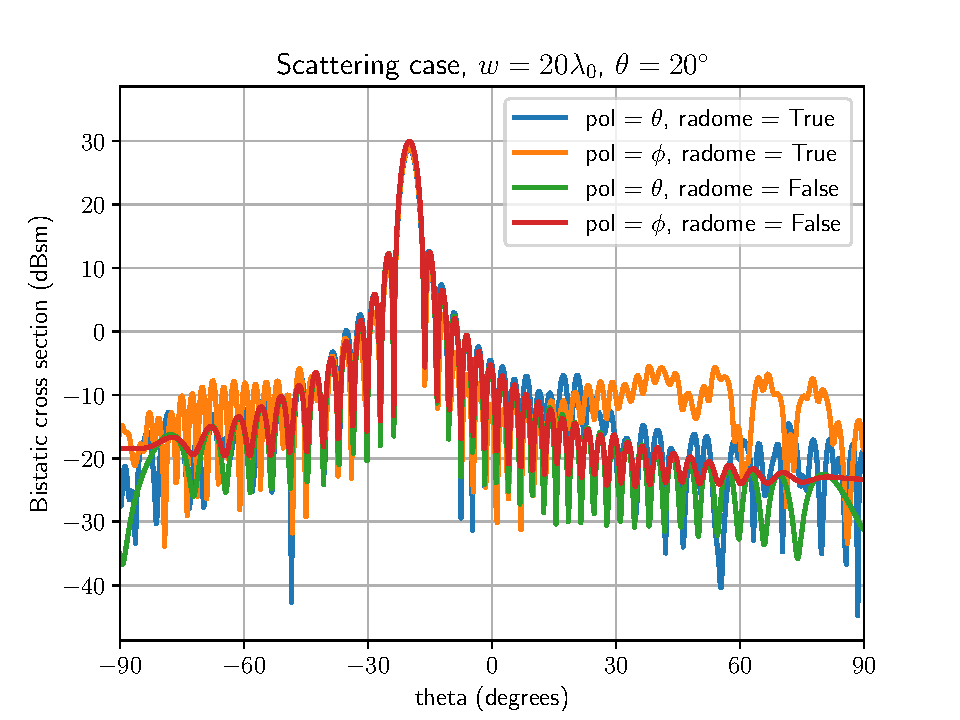
\includegraphics[width=\myfigwidth]{scattering_w20_theta20} &
      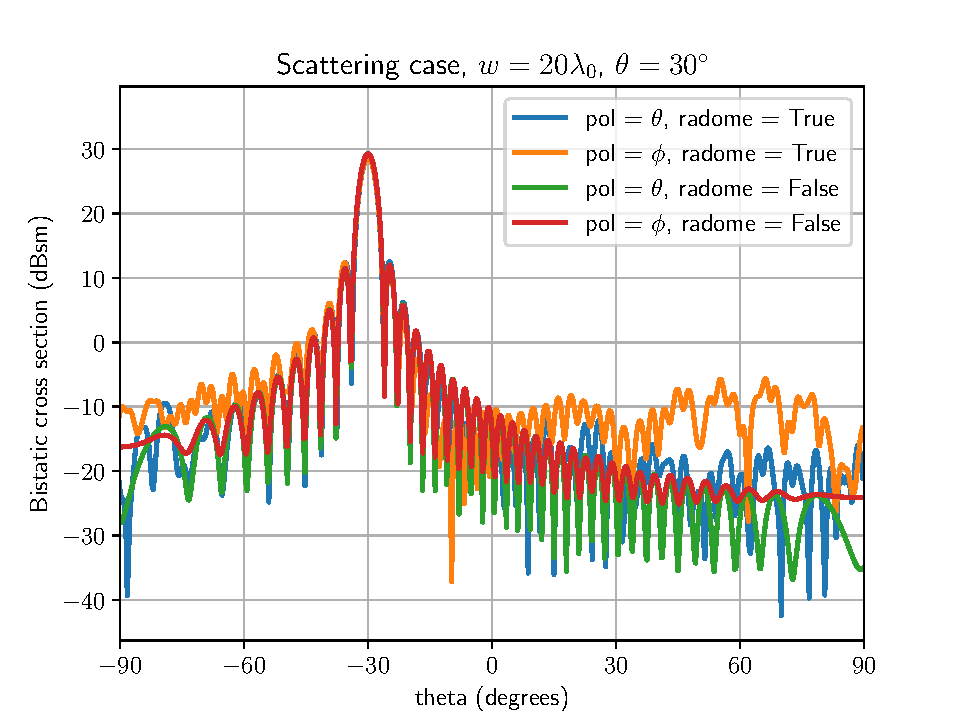
\includegraphics[width=\myfigwidth]{scattering_w20_theta30} \\
      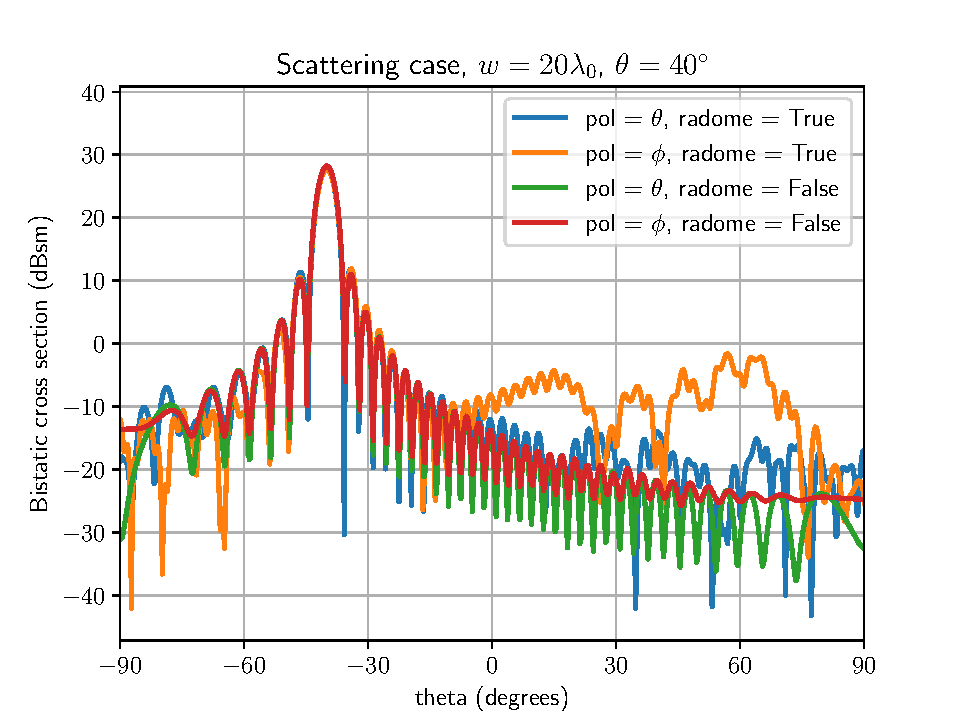
\includegraphics[width=\myfigwidth]{scattering_w20_theta40} &
      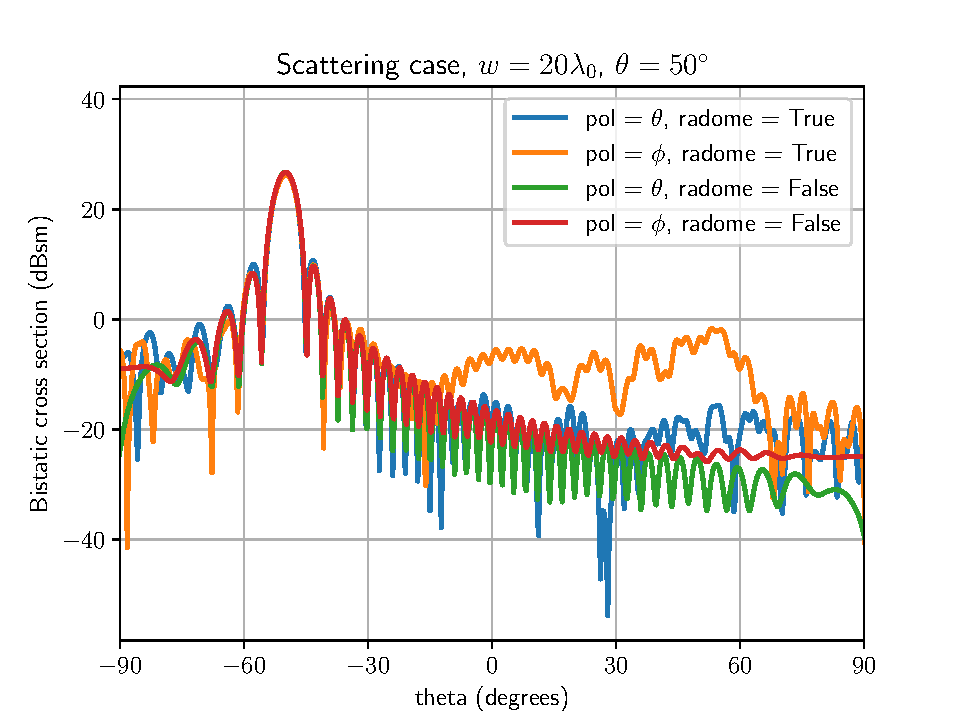
\includegraphics[width=\myfigwidth]{scattering_w20_theta50} 
    \end{tabular}
  \end{center}
  \caption{Scattering from antenna with and without radome, antenna
    width $w=20\lambda_{0}$.}
  \label{fig:scatteringw20}
\end{figure}

Finally, Figures~\ref{fig:transmissionw20} and
\ref{fig:transmissionw30} show the same results for a transmitting
antenna as Figure~\ref{fig:transmissionw10} but for antenna widths
$w=20\lambda_{0}$ and $30\lambda_{0}$, respectively. The reflection
lobe is clearly visible in both polarizations when the radome is
present. Also, the increased side lobe for the $\phi$-polarization
without radome remains, in particular for $w=30\lambda_{0}$ at
$\theta=40^{\circ}$ and $50^{\circ}$.

\begin{figure}
  \begin{center}
    \begin{tabular}{cc}
      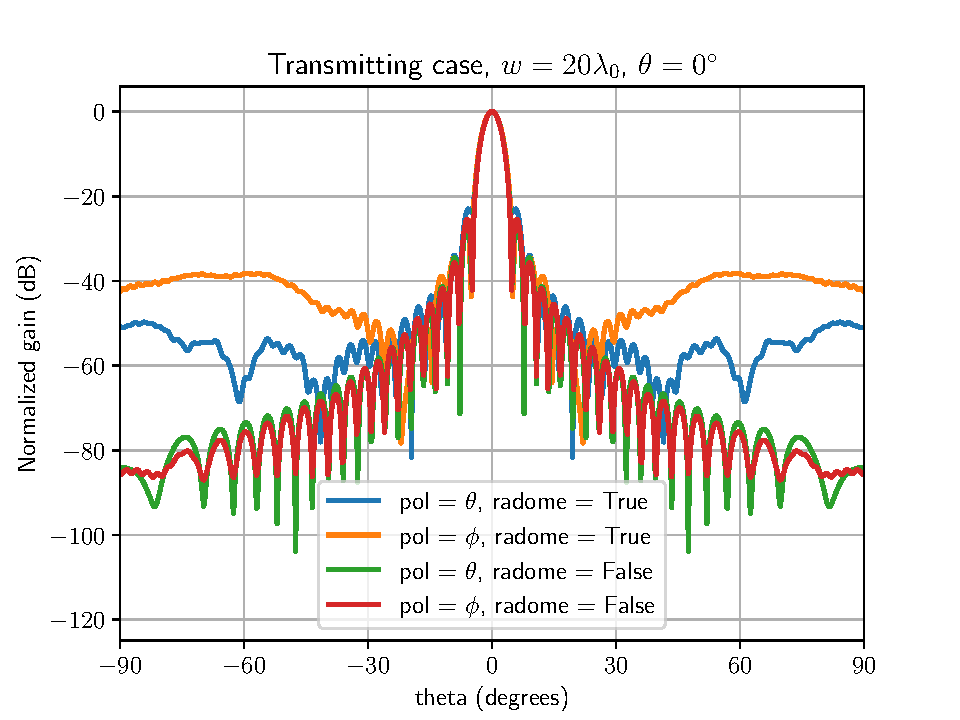
\includegraphics[width=\myfigwidth]{transmitting_w20_theta0} &
      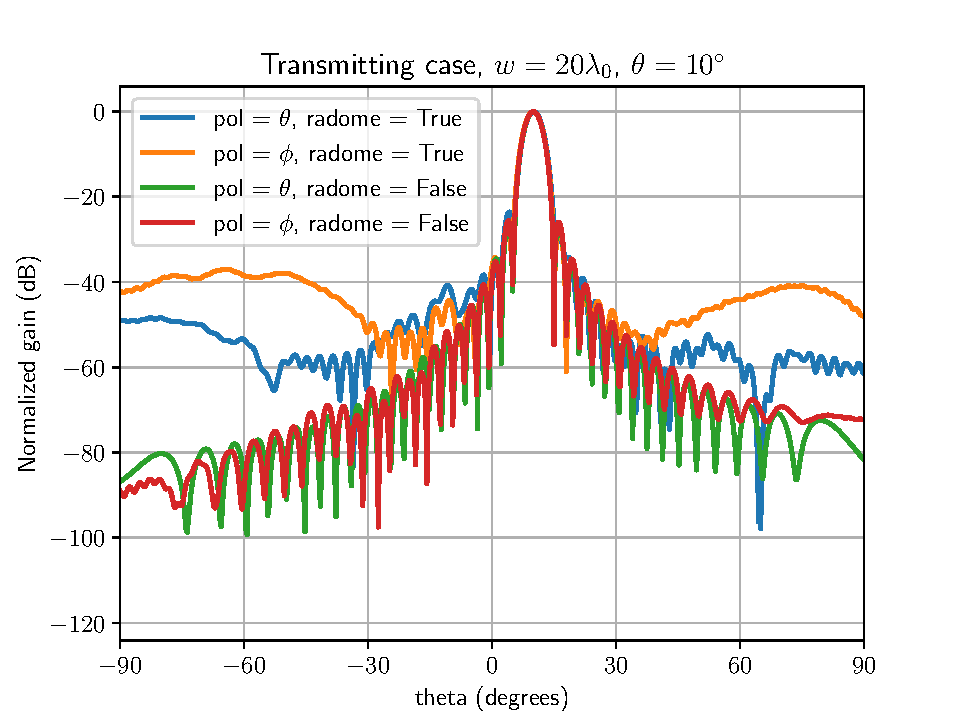
\includegraphics[width=\myfigwidth]{transmitting_w20_theta10} \\
      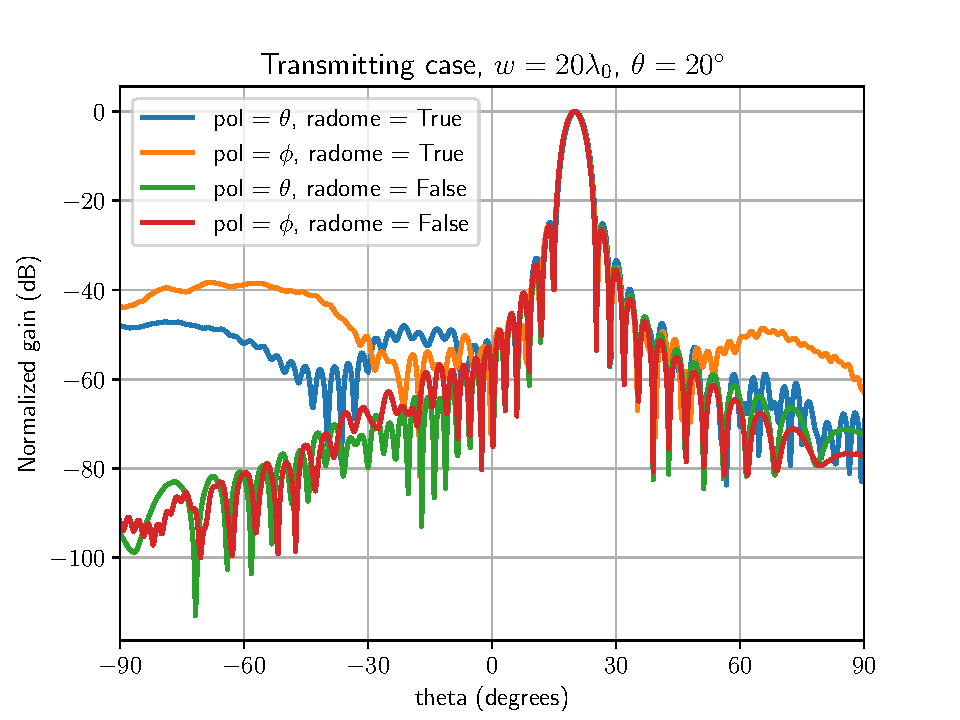
\includegraphics[width=\myfigwidth]{transmitting_w20_theta20} &
      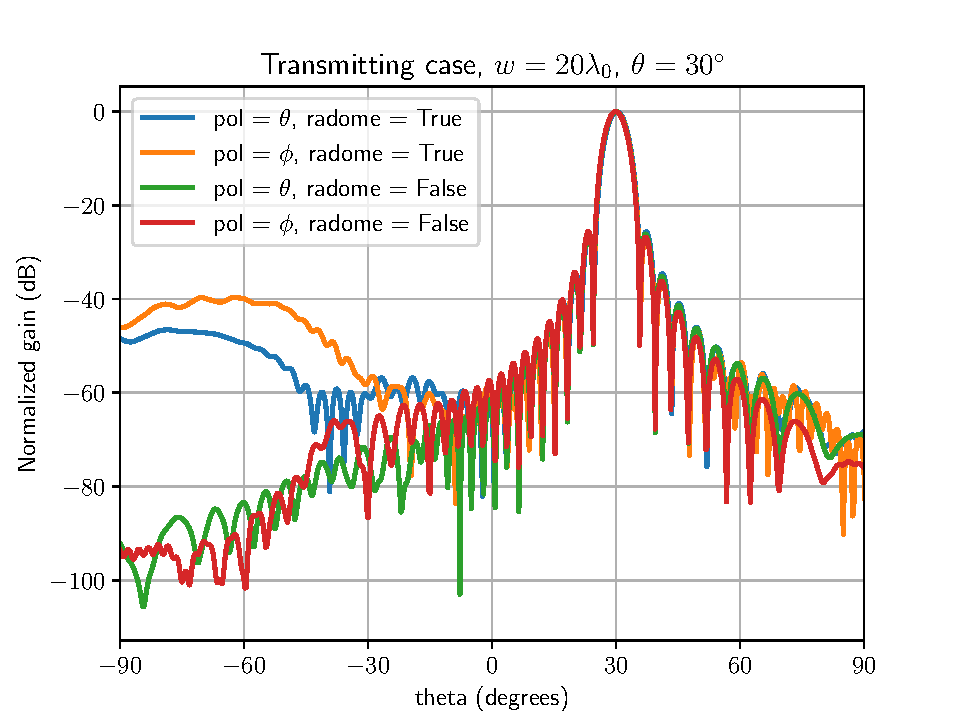
\includegraphics[width=\myfigwidth]{transmitting_w20_theta30} \\
      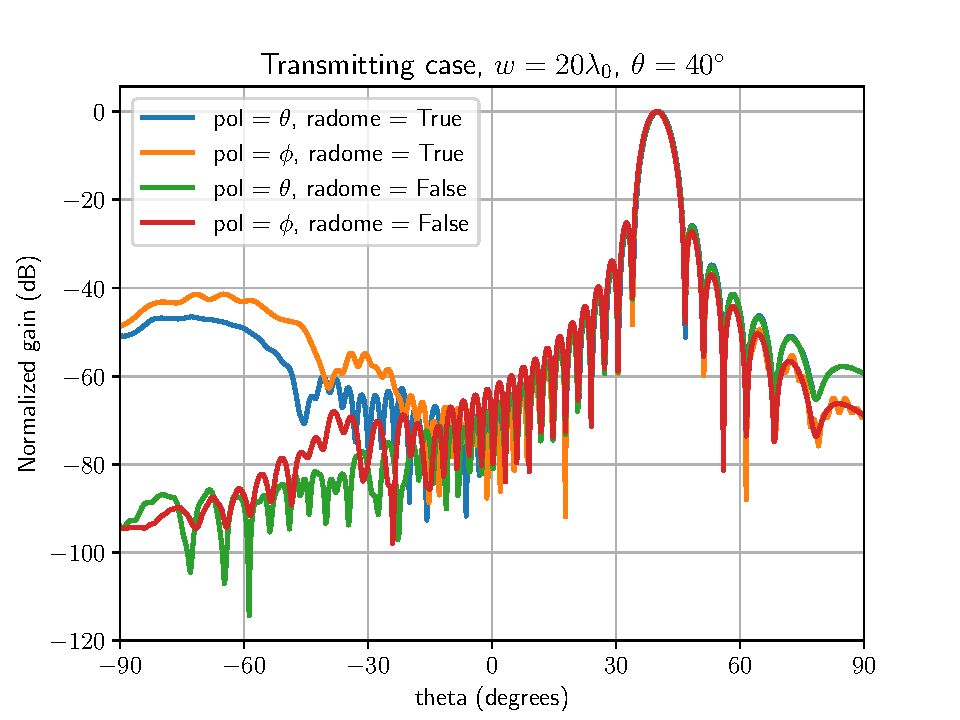
\includegraphics[width=\myfigwidth]{transmitting_w20_theta40} &
      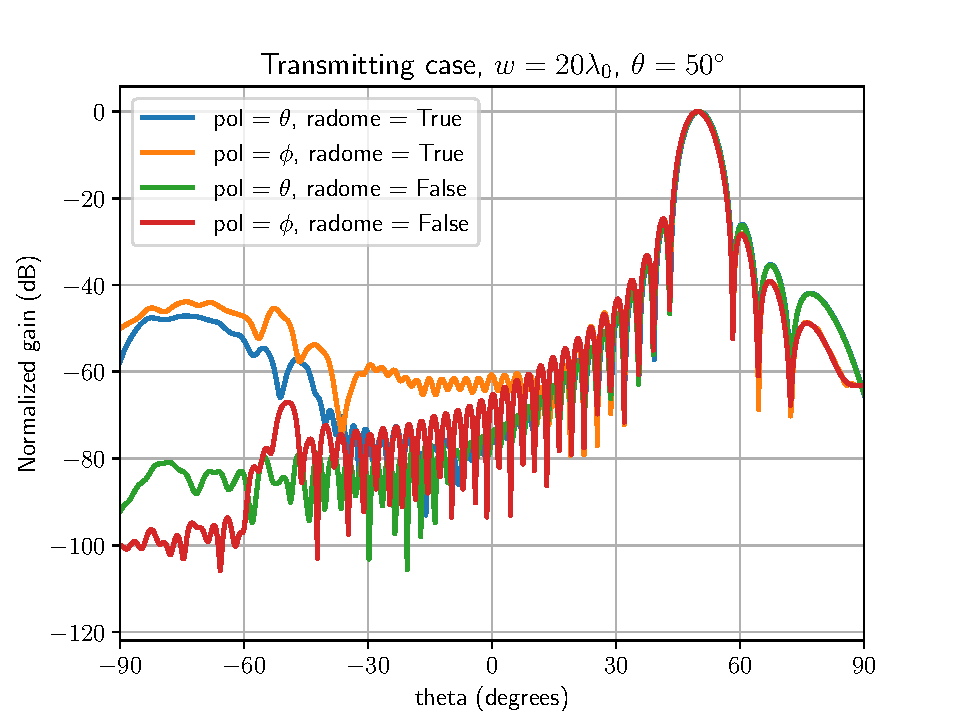
\includegraphics[width=\myfigwidth]{transmitting_w20_theta50} 
    \end{tabular}
  \end{center}
  \caption{Transmission from antenna with and without radome, antenna
    width $w=20\lambda_{0}$.}
  \label{fig:transmissionw20}
\end{figure}

\begin{figure}
  \begin{center}
    \begin{tabular}{cc}
      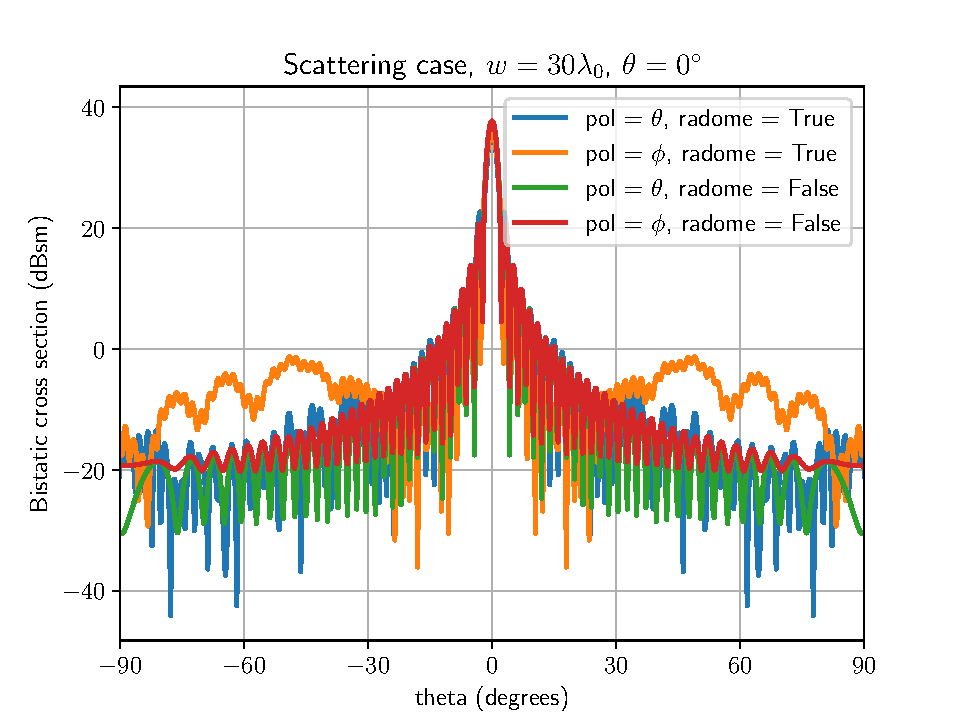
\includegraphics[width=\myfigwidth]{scattering_w30_theta0} &
      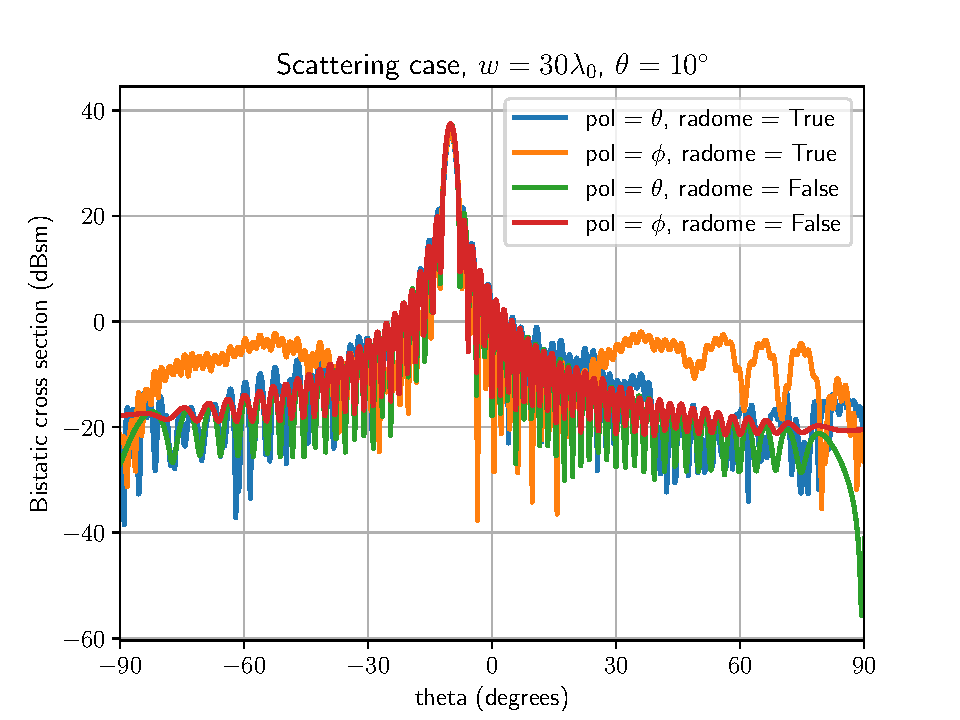
\includegraphics[width=\myfigwidth]{scattering_w30_theta10} \\
      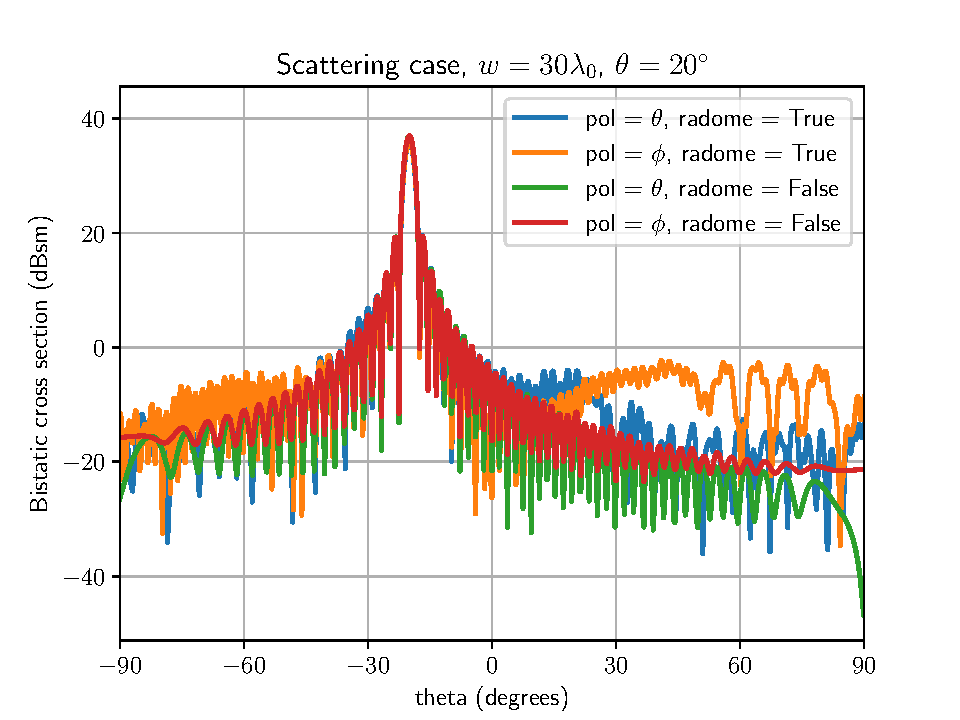
\includegraphics[width=\myfigwidth]{scattering_w30_theta20} &
      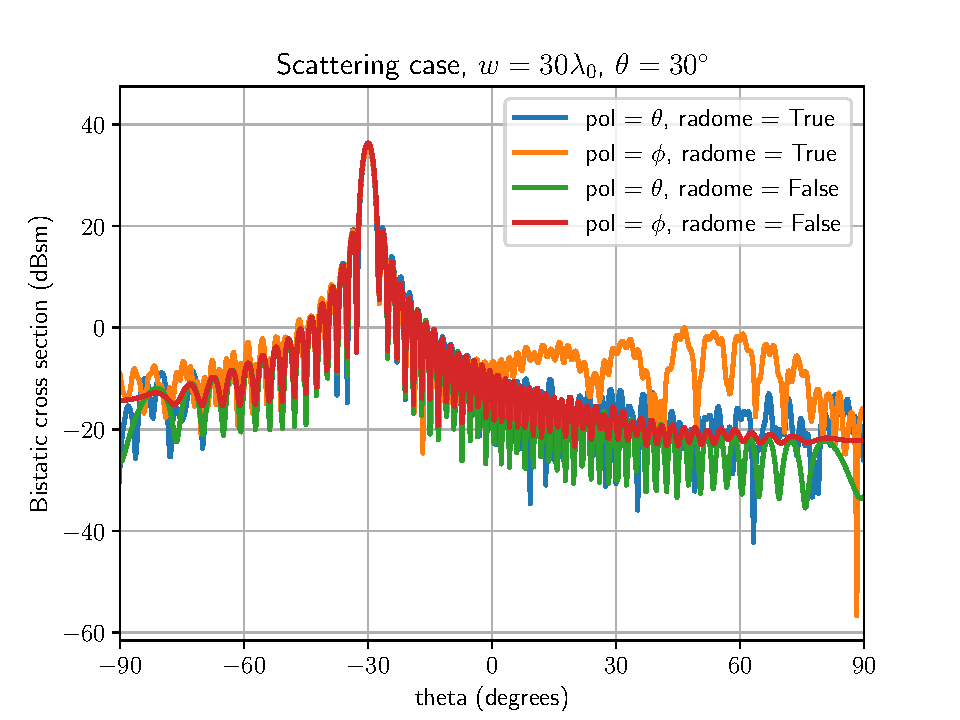
\includegraphics[width=\myfigwidth]{scattering_w30_theta30} \\
      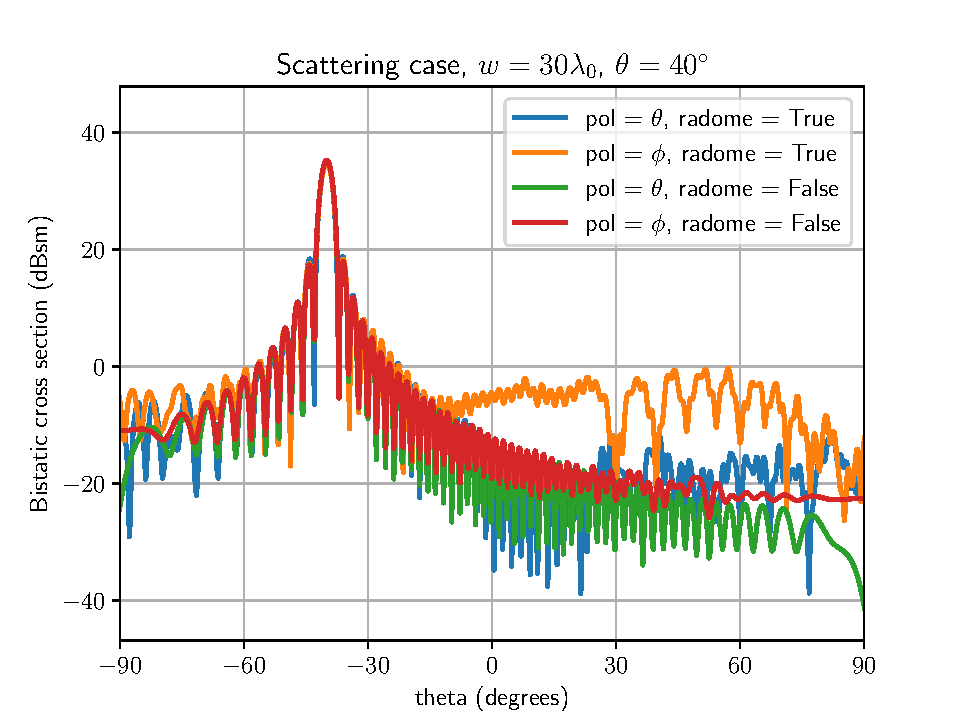
\includegraphics[width=\myfigwidth]{scattering_w30_theta40} &
      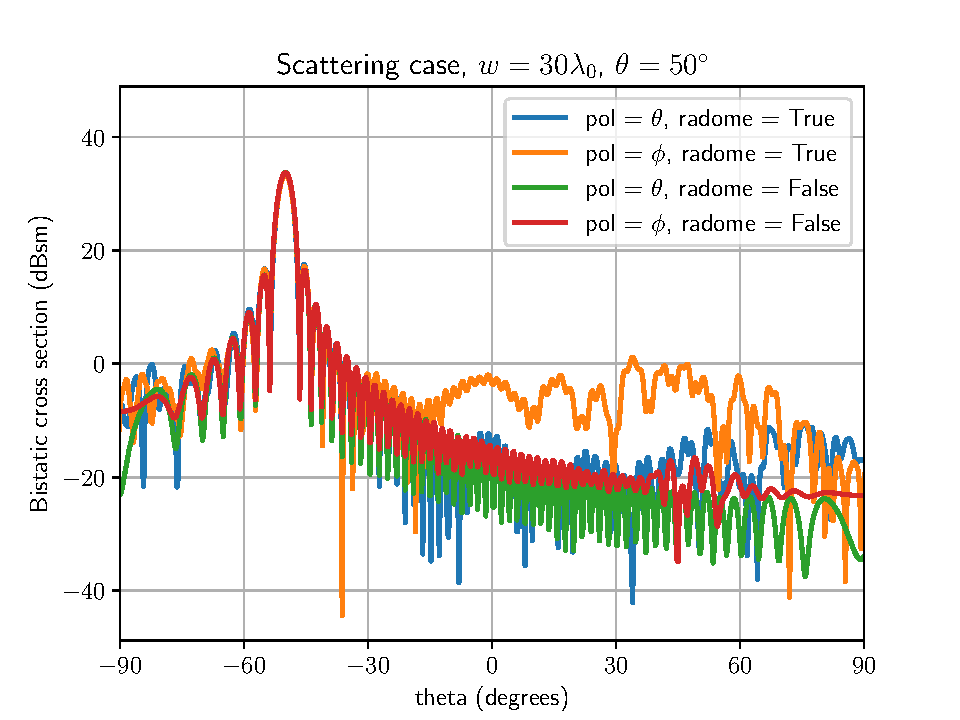
\includegraphics[width=\myfigwidth]{scattering_w30_theta50} 
    \end{tabular}
  \end{center}
  \caption{Scattering from antenna with and without radome, antenna
    width $w=30\lambda_{0}$.}
  \label{fig:scatteringw30}
\end{figure}

\begin{figure}
  \begin{center}
    \begin{tabular}{cc}
      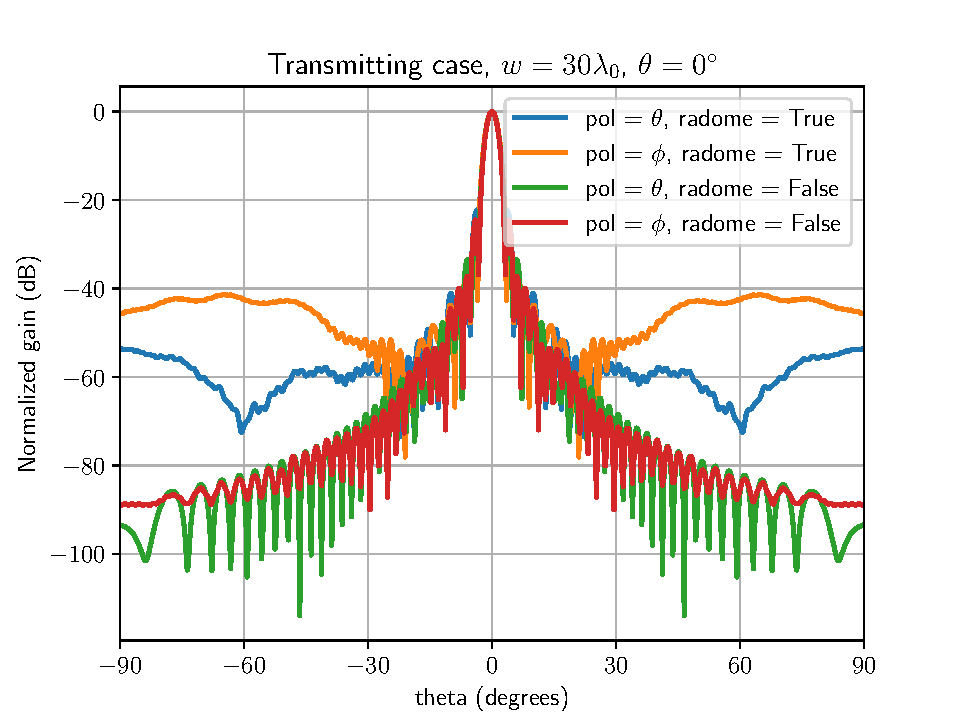
\includegraphics[width=\myfigwidth]{transmitting_w30_theta0} &
      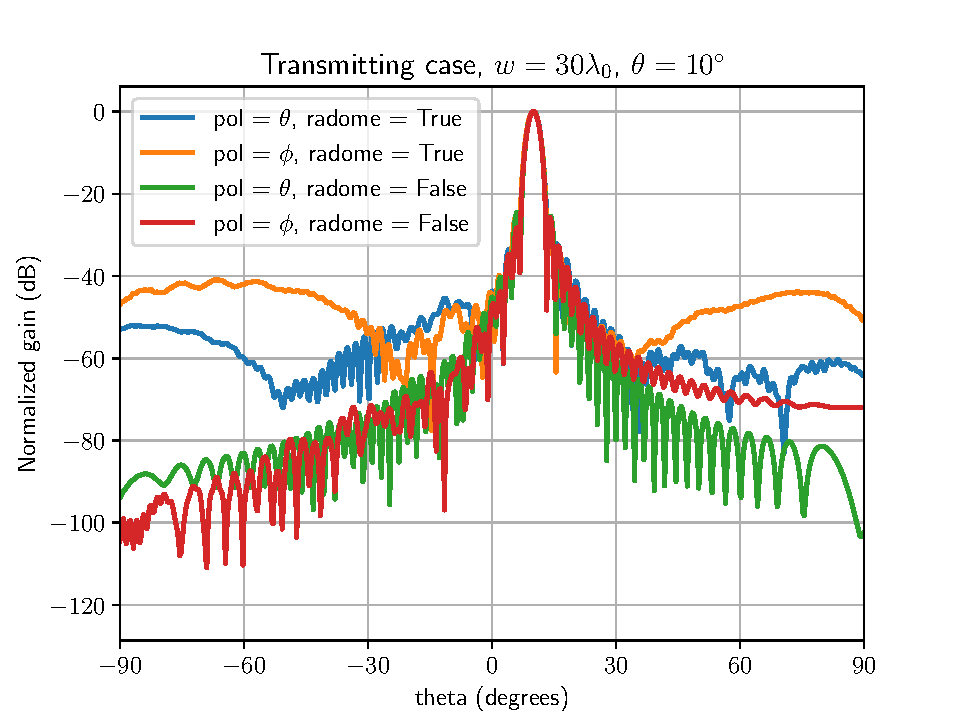
\includegraphics[width=\myfigwidth]{transmitting_w30_theta10} \\
      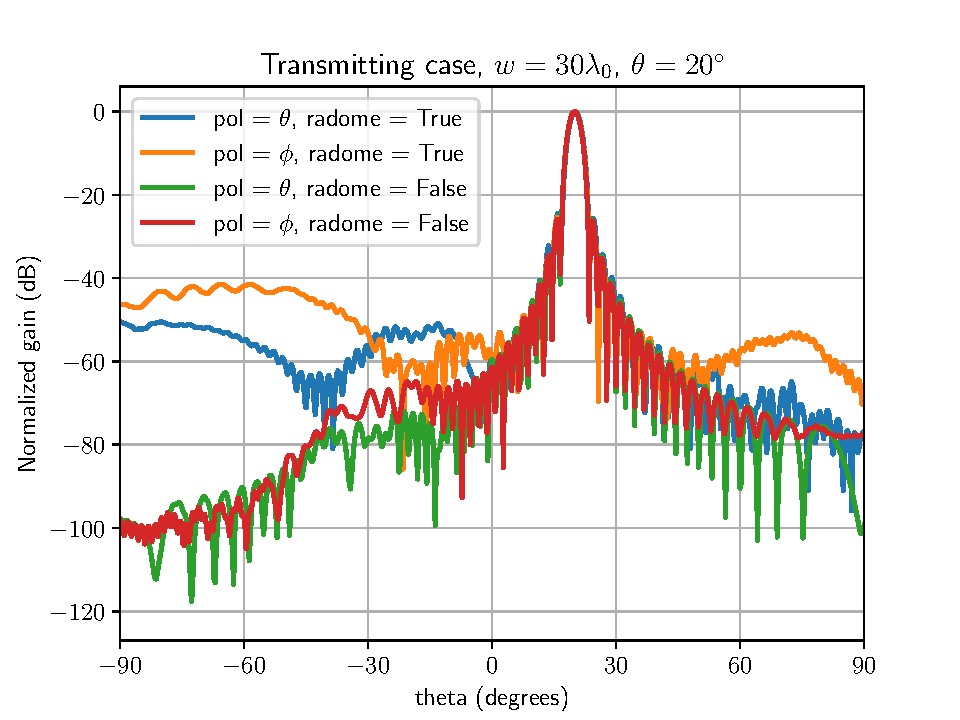
\includegraphics[width=\myfigwidth]{transmitting_w30_theta20} &
      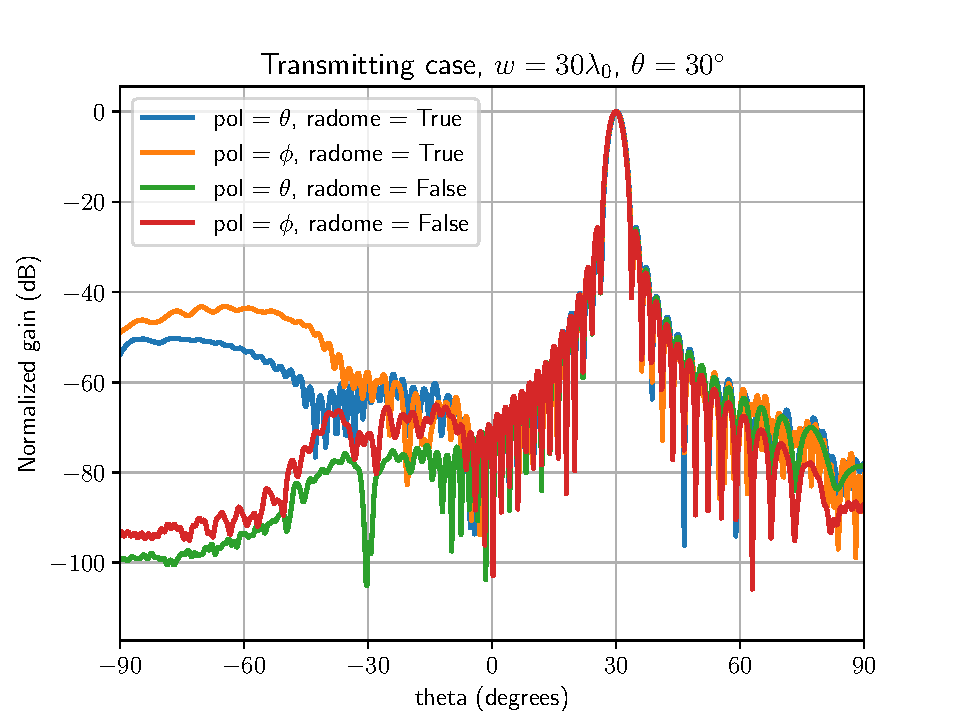
\includegraphics[width=\myfigwidth]{transmitting_w30_theta30} \\
      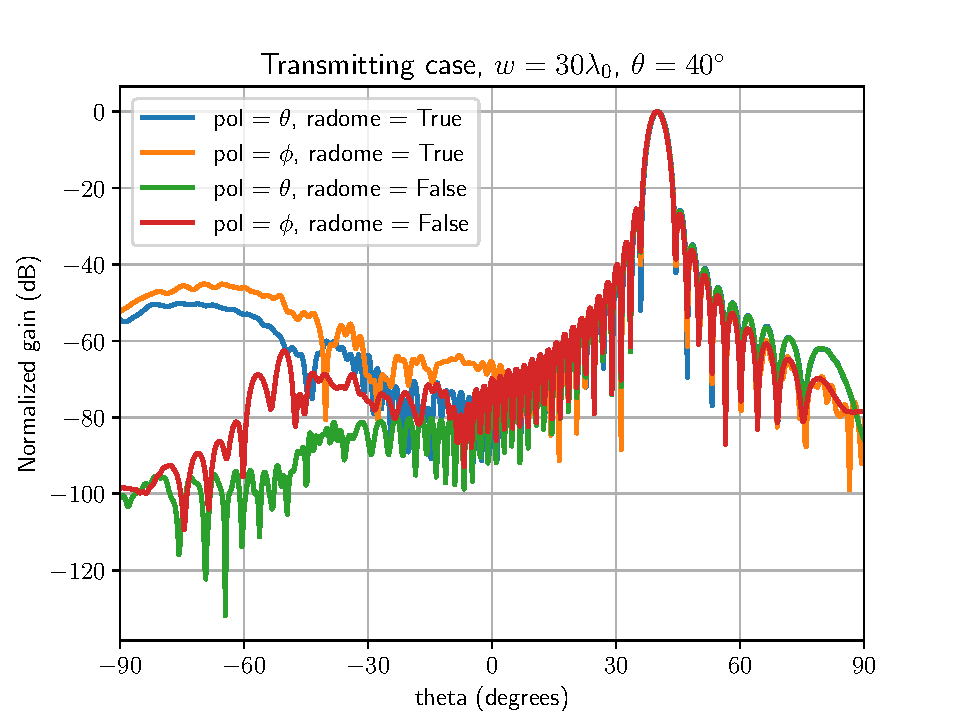
\includegraphics[width=\myfigwidth]{transmitting_w30_theta40} &
      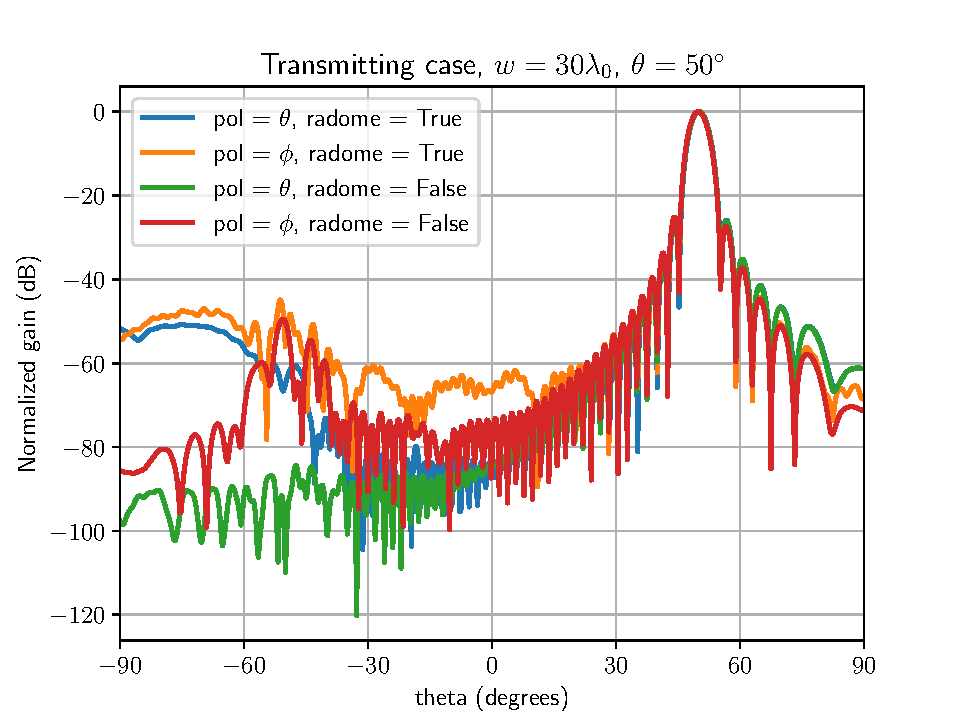
\includegraphics[width=\myfigwidth]{transmitting_w30_theta50} 
    \end{tabular}
  \end{center}
  \caption{Transmission from antenna with and without radome, antenna
    width $w=30\lambda_{0}$.}
  \label{fig:transmissionw30}
\end{figure}



\section{Conclusions}
\label{sec:conclusions}

We have described the theory and implementation of a finite elements
code for the simulation of a rotationally symmetric geometry, with the
purpose to provide benchmark cases for large radome simulations. The
code has been verified using scattering against PEC spheres and lossy
dielectric spheres using a Mie scattering code. The code can handle
excitation both with a transmitting antenna (with or without a
tapering for low side lobes), and an incident plane wave, with
arbitrary polarization. Both far field and near field data can be
considered, where the far field data can also be projected on the
spherical vector harmonics.

An application case has been illustrated, where a simple ogive-shaped
half-wavelength radome in various sizes has been simulated. An
increased bistatic scattering was observed for an incident plane wave
of $\phi$-polarization, and a reflection lobe in the transmitting case
was observed in both near field and far field data for both
polarizations. It should be emphasized that the radome studied has not
been optimized in any way, and the results presented here are only
intended to provide a reference case for other codes, not to represent
a good design.


\newpage

\appendix


\section{Perfectly matched layer}
\label{app:pml}

A perfectly matched layer (PML) region is used to absorb the outgoing
scattered field. We follow the dolfinx v0.7 demo on axisymmetric
scattering,\footnote{\url{https://docs.fenicsproject.org/dolfinx/main/python/demos/demo_axis.html}}
and consider a spherical region with stretched cylindrical coordinates
$\rho'(\rho,z)$, $z'(\rho,z)$, and $\varphi'=\varphi$. The coordinate
transformation has the Jacobian
\begin{equation}
  \mat{J} = \mat{A}^{-1} = \nabla\rv'(\rv) =
  \begin{pmatrix}
    \frac{\partial\rho'}{\partial\rho} & \frac{\partial z'}{\partial\rho} & 0 \\
    \frac{\partial\rho'}{\partial z} & \frac{\partial z'}{\partial z} & 0 \\
    0 & 0 & \frac{\rho'}{\rho}\frac{\partial\varphi'}{\partial\varphi}
  \end{pmatrix},
\end{equation}
and the PML material parameters are (with
$A=\operatorname{det}(\mat{A})$) 
\begin{align}
  \epsm_{\mrm{r,pml}} = A^{-1} \mat{A} \boldsymbol{\epsilon}_{\mrm{b}} \mat{A}^{\mrm{T}} \\
  \mum_{\mrm{r,pml}} = A^{-1} \mat{A} \boldsymbol{\mu}_{\mrm{b}} \mat{A}^{\mrm{T}}.
\end{align}
We consider stretching with a polynomial profile in spherical radius
$r=\sqrt{\rho^{2}+z^{2}}$ such that \cite[p. 663]{Taflove+etal2004}
\begin{align}
  \rho' &= \rho\left( 1 - \ju \frac{(n+1)\ln(1/R_{0})}{2k(r_{\mrm{pml}} - r_{\mrm{dom}})} \left(\frac{r-r_{\mrm{dom}}}{r_{\mrm{pml}} - r_{\mrm{dom}}}\right)^{n}\right) \\
  z' &= z\left( 1 - \ju \frac{(n+1)\ln(1/R_{0})}{2k(r_{\mrm{pml}} - r_{\mrm{dom}})} \left(\frac{r-r_{\mrm{dom}}}{r_{\mrm{pml}} - r_{\mrm{dom}}}\right)^{n}\right). 
\end{align}
where $R_{0}$ is the desired (amplitude scale) reflection coefficient
at normal incidence, and $n$ is the polynomial order. Suitable choices
are $R_{0} = 10^{-10}$ and $n=3$.

Another option is to stretch coordinates in $\rho$ and $z$
independently, which allows for structures parallel to the $z$-axis
extending into the PML (and hence considered infinite in this
direction). This is obtained by
\begin{align}
  \rho' &= \rho\left( 1 - \ju \frac{(n+1)\ln(1/R_{0})}{2k(\rho_{\mrm{pml}} - \rho_{\mrm{dom}})} \left(\frac{\rho-\rho_{\mrm{dom}}}{\rho_{\mrm{pml}} - \rho_{\mrm{dom}}}\right)^{n}\right) && \rho_{\mrm{dom}} < \rho < \rho_{\mrm{pml}} \\
  z' &= z\left( 1 - \ju \frac{(n+1)\ln(1/R_{0})}{2k(z_{\mrm{pml,t}} - z_{\mrm{dom,t}})} \left(\frac{z-z_{\mrm{dom,t}}}{z_{\mrm{pml,t}} - z_{\mrm{dom,t}}}\right)^{n}\right) && z_{\mrm{dom,t}} < z < z_{\mrm{pml,t}} \\
  z' &= z\left( 1 - \ju \frac{(n+1)\ln(1/R_{0})}{2k(z_{\mrm{dom,b}} - z_{\mrm{pml,b}})} \left(\frac{z_{\mrm{dom,b}}-z}{z_{\mrm{dom,b}} - z_{\mrm{pml,b}}}\right)^{n}\right) && z_{\mrm{pml,b}} < z < z_{\mrm{dom,b}} 
\end{align}
and unstretched coordinates otherwise. In the overlap regions, both
$\rho'$ and $z'$ are stretched by the formulas above. We can write a
stretching function (note the use of the absolute value in order to
have positive quantities regardless of the sign of
$x_{\mrm{pml}}-x_{\mrm{dom}}$)
\begin{equation}
  s(x,x_{\mrm{dom}},x_{\mrm{pml}}) = 1 - \ju\frac{(n+1)\ln(1/R_{0})}{2k|x_{\mrm{pml}} - x_{\mrm{dom}}|} \left(\frac{x-x_{\mrm{dom}}}{x_{\mrm{pml}} - x_{\mrm{dom}}}\right)^{n},
\end{equation}
where $x$ denotes the coordinate normal to the PML, with
$x_{\mrm{dom}}$ and $x_{\mrm{pml}}$ denoting the coordinates at the
end of the domain and the end of the PML, respectively. Hence, a
spherical PML has
\begin{align}
  \rho' &= \rho s(r,r_{\mrm{dom}},r_{\mrm{pml}}) && r_{\mrm{dom}} < r < r_{\mrm{pml}} \\
  z' &= z s(r,r_{\mrm{dom}},r_{\mrm{pml}}) && r_{\mrm{dom}} < r < r_{\mrm{pml}}
\end{align}
with $r = \sqrt{\rho^{2} + z^{2}}$, whereas a cylindrical PML has
\begin{align}
  \rho' &= \rho s(\rho,\rho_{\mrm{dom}},\rho_{\mrm{pml}}) && \rho_{\mrm{dom}} < \rho < \rho_{\mrm{pml}} \\
  z' &= z s(z,z_{\mrm{dom,t}},z_{\mrm{pml,t}}) && z_{\mrm{dom,t}} < z < z_{\mrm{pml,t}} \\
  z' &= z s(z,z_{\mrm{dom,b}},z_{\mrm{pml,b}}) && z_{\mrm{pml,t}} < z < z_{\mrm{dom,t}}. 
\end{align}
We note that this is not strictly the correct scaling since $s$
depends on the coordinates, we should have
$s=\partial \rho'/\partial\rho$ etc. However, it seems to work in
practice.


\section{Plane wave in cylindrical coordinates}
\label{app:planewave}

An incident plane wave is described by
\begin{equation}
  \Ev_{\mrm{b}}(\rv) = \Ev_{0}\eu^{-\ju\kv\cdot\rv},
\end{equation}
where
\begin{equation}
  \kv = k(\xuv\sin\theta\cos\phi + \yuv\sin\theta\sin\phi + \zuv\cos\theta),
\end{equation}
The Cartesian unit vectors can be written in terms of the cylindrical as
\begin{align}
  \xuv &= \rhouv\cos\varphi - \varphiuv\sin\varphi \\
  \yuv &= \rhouv\sin\varphi + \varphiuv\cos\varphi \\
  \zuv &= \zuv,
\end{align}
implying
\begin{equation}
  \kv\cdot\rv = k\rho\sin\theta(\cos\phi\cos\varphi + \sin\phi\sin\varphi) + kz\cos\theta 
  = k\rho\sin\theta\cos(\varphi-\phi) + kz\cos\theta.
\end{equation}
Using the Jacobi-Anger expansion \cite[9.1.42--45]{Abramowitz+Stegun1970}
\begin{equation}
  \eu^{\ju z\cos\varphi} = \sum_{n=-\infty}^{\infty}\ju^{n}\BesselJ_{n}(z)\eu^{\ju n\varphi},
\end{equation}
we can then write
\begin{equation}
  \eu^{-\ju\kv\cdot\rv} = \eu^{-\ju k\rho\sin\theta\cos(\varphi-\phi)}\eu^{-\ju kz\cos\theta} = \eu^{-\ju kz\cos\theta} \sum_{n=-\infty}^{\infty}(-\ju)^{n}\BesselJ_{n}(k\rho\sin\theta)\eu^{-\ju n(\varphi-\phi)}.
\end{equation}
The polarization of the wave is
\begin{equation}
  \Ev_{0} = \thetauv E_{\theta} + \phiuv E_{\phi},
\end{equation}
where the unit vectors are
\begin{multline}
  \thetauv = \cos\theta\cos\phi\xuv + \cos\theta\sin\phi\yuv - \sin\theta\zuv \\
  = \cos\theta(\cos\phi\cos\varphi + \sin\phi\sin\varphi)\rhouv + \cos\theta(-\cos\phi\sin\varphi + \sin\phi\cos\varphi)\varphiuv - \sin\theta\zuv \\
  = \cos\theta\cos(\varphi-\phi)\rhouv - \cos\theta\sin(\varphi-\phi)\varphiuv - \sin\theta\zuv
\end{multline}
and
\begin{multline}
  \phiuv = -\sin\phi\xuv + \cos\phi\yuv = (-\sin\phi\cos\varphi + \cos\phi\sin\varphi)\rhouv + (\sin\phi\sin\varphi + \cos\phi\cos\varphi)\varphiuv \\
  = \sin(\varphi-\phi)\rhouv + \cos(\varphi-\phi)\varphiuv.
\end{multline}
Using Euler's formula we have
\begin{equation}
  \cos(\varphi-\phi) = \frac{\eu^{\ju(\varphi-\phi)}+\eu^{-\ju(\varphi-\phi)}}{2} \quad\text{and}\quad \sin(\varphi-\phi) = \frac{\eu^{\ju(\varphi-\phi)}-\eu^{-\ju(\varphi-\phi)}}{2\ju},
\end{equation}
and the final version of the plane wave expansion is
\begin{multline}
  \Ev_{0}\eu^{-\ju\kv\cdot\rv} = E_{\theta}\eu^{-\ju kz\cos\theta} \Bigg\{ \left[ \sum_{n=-\infty}^{\infty}(-\ju)^{n}\BesselJ_{n}(k\rho\sin\theta)\frac{1}{2}(\eu^{-\ju (n-1)(\varphi-\phi)} + \eu^{-\ju (n+1)(\varphi-\phi)}) \right]\cos\theta\rhouv \\
  + \left[ \sum_{n=-\infty}^{\infty}(-\ju)^{n}\BesselJ_{n}(k\rho\sin\theta) \frac{1}{2\ju}(\eu^{-\ju (n-1)(\varphi-\phi)} - \eu^{-\ju (n+1)(\varphi-\phi)}) \right](-\cos\theta)\varphiuv \\
  + \left[ \sum_{n=-\infty}^{\infty}(-\ju)^{n}\BesselJ_{n}(k\rho\sin\theta)\eu^{-\ju n(\varphi-\phi)}\right](-\sin\theta)\zuv \Bigg\} \\
  + E_{\phi}\eu^{-\ju kz\cos\theta} \Bigg\{ \left[ \sum_{n=-\infty}^{\infty}(-\ju)^{n}\BesselJ_{n}(k\rho\sin\theta) \frac{1}{2\ju}(\eu^{-\ju (n-1)(\varphi-\phi)} - \eu^{-\ju (n+1)(\varphi-\phi)}) \right]\rhouv \\
  + \left[ \sum_{n=-\infty}^{\infty}(-\ju)^{n}\BesselJ_{n}(k\rho\sin\theta)\frac{1}{2}(\eu^{-\ju (n-1)(\varphi-\phi)} + \eu^{-\ju (n+1)(\varphi-\phi)}) \right] \varphiuv \Bigg\}.
\end{multline}
Rewriting in terms of azimuthal modes, we find
\begin{multline}
  \Ev_{0}\eu^{-\ju\kv\cdot\rv} = E_{\theta}\eu^{-\ju kz\cos\theta} \Bigg\{ \sum_{n=-\infty}^{\infty} \frac{1}{2}\left[ (-\ju)^{n+1}\BesselJ_{n+1}(k\rho\sin\theta) + (-\ju)^{n-1}\BesselJ_{n-1}(k\rho\sin\theta)\right] \eu^{-\ju n(\varphi-\phi)} \cos\theta\rhouv \\
  + \sum_{n=-\infty}^{\infty} \frac{1}{2\ju}\left[ (-\ju)^{n+1}\BesselJ_{n+1}(k\rho\sin\theta) - (-\ju)^{n-1}\BesselJ_{n-1}(k\rho\sin\theta)\right] \eu^{-\ju n(\varphi-\phi)} (-\cos\theta)\varphiuv \\
  + \sum_{n=-\infty}^{\infty}(-\ju)^{n}\BesselJ_{n}(k\rho\sin\theta)\eu^{-\ju n(\varphi-\phi)} (-\sin\theta)\zuv \Bigg\} \\
  + E_{\phi}\eu^{-\ju kz\cos\theta} \Bigg\{ \sum_{n=-\infty}^{\infty} \frac{1}{2\ju} \left[ (-\ju)^{n+1}\BesselJ_{n+1}(k\rho\sin\theta) - (-\ju)^{n-1}\BesselJ_{n-1}(k\rho\sin\theta)\right] \eu^{-\ju n(\varphi-\phi)} \rhouv \\
  + \sum_{n=-\infty}^{\infty} \frac{1}{2} \left[ (-\ju)^{n+1}\BesselJ_{n+1}(k\rho\sin\theta) + (-\ju)^{n-1}\BesselJ_{n-1}(k\rho\sin\theta) \right] \eu^{-\ju n(\varphi-\phi)} \varphiuv \Bigg\},
  \label{eq:planewave}
\end{multline}
which is our final expression. This expression can also be used to
compute an antenna excitation $\Ev_{\mrm{a}}$: simply evaluate it on
the antenna surface, possibly multiplied by an amplitude taper.

\section{Computation of far field amplitudes}
\label{app:farfield}

In this Appendix, we give explicit derivations of how the far field
amplitudes used in the computational examples can be derived. The
general setup of solving Maxwell's equations in a rotationally
symmetric geometry is provided in Section~\ref{sec:rotational}. There,
it is seen that the fields can be represented in cylindrical
coordinates $(\rho,\varphi,z)$ as
\begin{align}
  \Ev(\rv) &= \sum_{m=-\infty}^{\infty} \left[E_{\rho}^{(m)}(\rho,z)\rhouv + E_{\varphi}^{(m)}(\rho,z)\varphiuv + E_{z}^{(m)}(\rho,z)\zuv \right] \eu^{-\ju m\varphi} \\
  \Hv(\rv) &= \sum_{m=-\infty}^{\infty} \left[H_{\rho}^{(m)}(\rho,z)\rhouv + H_{\varphi}^{(m)}(\rho,z)\varphiuv + H_{z}^{(m)}(\rho,z)\zuv \right] \eu^{-\ju m\varphi}.
\end{align}
In this Appendix, we demonstrate how to solve the azimuthal part of
the far field integral 
\begin{equation}
  \Fv(\kuv) = \frac{\ju k}{4\pi} \kuv\times \iint_{S} \left[ \Ev(\rv)\times\nuv + \eta_{0}\kuv\times(\nuv\times\Hv(\rv)) \right] \eu^{\ju k\kuv\cdot\rv} \diff S
\end{equation}
for arbitrary azimuthal mode index $m$. The radiation direction $\kuv$
is parameterized by the standard polar angle $\theta$ and azimuth
angle $\phi$.

The fields $\Ev^{(m)}(\rho,z)$ and $\Hv^{(m)}(\rho,z)$ depend only on
$\rho$ and $z$, whereas the $\varphi$-dependence is in a factor
$\eu^{-\ju m\varphi}$. Hence, the far field integrals to be computed
are proportional to
\begin{equation}
  \int_{\vec{\rho}\in\gamma}\int_{\varphi=0}^{2\pi} [\Ev^{(m)}\times\nuv] \eu^{\ju(\kv\cdot\rv - m\varphi)} \rho\diff\varphi\diff\ell \quad\text{and}\quad \int_{\vec{\rho}\in\gamma} \int_{\varphi=0}^{2\pi} [\nuv\times\Hv^{(m)}] \eu^{\ju(\kv\cdot\rv - m\varphi)} \rho\diff\varphi\diff\ell,
\end{equation}
where $\gamma$ is the curve in the $\rho$-$z$ plane where the integral
is to be computed, $\rho$ and $z$ are coordinates on this curve, with
$\diff\ell$ as a line element.  The unit normal vector is
$\nuv = n_{\rho}\rhouv+n_{z}\zuv$, meaning the electric and magnetic
tangential fields are (using $\rhouv\times\varphiuv = \zuv$)
\begin{align}
  \Ev^{(m)}\times\nuv &= (n_{\rho}E_{z}^{(m)} - n_{z}E_{\rho}^{(m)})\varphiuv - n_{\rho}E_{\varphi}^{(m)}\zuv + n_{z}E_{\varphi}^{(m)}\rhouv \\
  \nuv\times\Hv^{(m)} &= (-n_{\rho}H_{z}^{(m)} + n_{z}H_{\rho}^{(m)})\varphiuv + n_{\rho}H_{\varphi}^{(m)}\zuv - n_{z}H_{\varphi}^{(m)}\rhouv.
\end{align}
The unit vectors are
\begin{align}
  \rhouv &= \xuv\cos\varphi + \yuv\sin\varphi \\
  \varphiuv &= -\xuv\sin\varphi+\yuv\cos\varphi,
\end{align}
meaning the tangential fields are
\begin{align}
  \Ev^{(m)}\times\nuv &= [n_{z}E_{\varphi}^{(m)}\cos(\varphi) -(n_{\rho}E_{z}^{(m)} - n_{z}E_{\rho}^{(m)})\sin(\varphi)]\xuv \\
  &\quad + [n_{z}E_{\varphi}^{(m)}\sin(\varphi) + (n_{\rho}E_{z}^{(m)} - n_{z}E_{\rho}^{(m)})\cos(\varphi)]\yuv - n_{\rho}E_{\varphi}^{(m)}\zuv \\
  \nuv\times\Hv^{(m)} &= - [n_{z}H_{\varphi}^{(m)}\cos(\varphi) - (n_{\rho}H_{z}^{(m)} - n_{z}H_{\rho}^{(m)})\sin(\varphi)]\xuv \\
  &\quad - [n_{z}H_{\varphi}^{(m)}\sin(\varphi) + (n_{\rho}H_{z}^{(m)} - n_{z}H_{\rho}^{(m)})\cos(\varphi)]\yuv + n_{\rho}H_{\varphi}^{(m)}\zuv.
\end{align}
The phase factor is
\begin{equation}
  \eu^{\ju(\kv\cdot\rv - m\varphi)} = \eu^{\ju(\kv\cdot(\rho\rhouv+z\zuv) - m\varphi)} = \eu^{\ju(k\rho\sin\theta\cos(\varphi-\phi) - m\varphi)}\eu^{\ju kz\cos\theta},
\end{equation}
where we used
$\kv\cdot\rv = k\rho\sin\theta\cos(\varphi-\phi) + kz\cos\theta$, with
$\kv = k[\sin\theta(\cos\phi\xuv + \sin\phi\yuv) + \cos\theta\zuv]$.
Thus, the typical azimuth integrals to be computed are:
\begin{align}
  \int_{0}^{2\pi} \eu^{\ju(k\rho\sin\theta\cos(\varphi-\phi) - m\varphi)} \diff\varphi
  &\stackrel{\varphi'=\varphi-\phi+\pi/2}{=} \int_{0}^{2\pi} \eu^{\ju(k\rho\sin\theta\cos(\varphi'-\pi/2) - m(\varphi'+\phi-\pi/2))} \diff\varphi' \notag \\
  &= \eu^{-\ju m(\phi-\pi/2)} \int_{-\pi}^{\pi} \eu^{\ju(k\rho\sin\theta\sin(\varphi') - m\varphi')} \diff\varphi' \notag \\
  &= \eu^{-\ju m\phi} \ju^{m}2\pi\BesselJ_{m}(k\rho\sin\theta) \notag \\
  &= 2\pi\ju^{m}\eu^{-\ju m\phi}A_{m} \\
  \int_{0}^{2\pi} \sin(\varphi)\eu^{\ju(k\rho\cos(\varphi-\phi) - m\varphi} \diff\varphi &= \frac{1}{2\ju} \Bigg[ \int_{0}^{2\pi} \eu^{\ju(k\rho\sin\theta\cos(\varphi-\phi) - (m-1)\varphi)} \diff\varphi \notag \\
  &\quad - \int_{0}^{2\pi} \eu^{\ju(k\rho\sin\theta\cos(\varphi-\phi) - (m+1)\varphi)} \diff\varphi \Bigg] \notag \\
  &= \frac{1}{2\ju} \Big[ \eu^{-\ju(m-1)\phi}\ju^{m-1}2\pi\BesselJ_{m-1}(k\rho\sin\theta) \notag \\
  &\quad - \eu^{-\ju(m+1)\phi}\ju^{m+1}2\pi\BesselJ_{m+1}(k\rho\sin\theta) \Big] \notag \\
  &= 2\pi\ju^{m}\eu^{-\ju m\phi} \frac{1}{2\ju}\left[ \eu^{\ju\phi}\ju^{-1}\BesselJ_{m-1}(k\rho\sin\theta) - \eu^{-\ju\phi}\ju\BesselJ_{m+1}(k\rho\sin\theta) \right] \notag \\
  &= -2\pi\ju^{m}\eu^{-\ju m\phi} \frac{1}{2}\left[ \eu^{\ju\phi}\BesselJ_{m-1}(k\rho\sin\theta) + \eu^{-\ju\phi}\BesselJ_{m+1}(k\rho\sin\theta) \right] \notag \\
  &= -2\pi\ju^{m}\eu^{-\ju m\phi}S_{m} \\
  \int_{0}^{2\pi} \cos(\varphi)\eu^{\ju k\rho\cos(\varphi-\phi) - m\varphi} \diff\varphi &= \frac{1}{2} \Bigg[ \int_{0}^{2\pi} \eu^{\ju(k\rho\sin\theta\cos(\varphi-\phi) - (m-1)\varphi)} \diff\varphi \notag \\
  &\quad + \int_{0}^{2\pi} \eu^{\ju(k\rho\sin\theta\cos(\varphi-\phi) - (m+1)\varphi)} \diff\varphi \Bigg] \notag \\
  &= \frac{1}{2} \Big[ \eu^{-\ju(m-1)\phi}\ju^{m-1}2\pi\BesselJ_{m-1}(k\rho\sin\theta) \notag \\
  &\quad + \eu^{-\ju(m+1)\phi}\ju^{m+1}2\pi\BesselJ_{m+1}(k\rho\sin\theta) \Big] \notag \\
  &= 2\pi\ju^{m}\eu^{-\ju m\phi} \frac{1}{2} \left[ \eu^{\ju\phi}\ju^{-1}\BesselJ_{m-1}(k\rho\sin\theta) + \eu^{-\ju\phi}\ju\BesselJ_{m+1}(k\rho\sin\theta) \right] \notag \\
  &= -2\pi\ju^{m}\eu^{-\ju m\phi} \frac{\ju}{2} \left[ \eu^{\ju\phi}\BesselJ_{m-1}(k\rho\sin\theta) - \eu^{-\ju\phi}\BesselJ_{m+1}(k\rho\sin\theta) \right] \notag \\
  &= -2\pi\ju^{m}\eu^{-\ju m\phi}C_{m},
\end{align}
where we used the representation \cite[9.1.21]{Abramowitz+Stegun1970}
\begin{equation}
  \BesselJ_{m}(z) = \frac{1}{\pi}\int_{0}^{\pi}\cos(z\sin\theta-m\theta)\diff\theta = \frac{1}{2\pi}\int_{-\pi}^{\pi}\eu^{\ju(z\sin\theta-m\theta)}\diff\theta = \frac{1}{2\pi}\int_{0}^{2\pi}\eu^{\ju(z\sin\theta-m\theta)}\diff\theta,
\end{equation}
where $m$ is a positive integer or zero. Thus, after integration over
$\varphi$, we have (premultiplying with the factor
$1/(2\pi\ju^{m}\eu^{\ju(kz\cos\theta-m\phi)})$ for simplicity)
\begin{multline}
  \frac{1}{2\pi\ju^{m}\eu^{\ju(kz\cos\theta-m\phi)}}\int_{0}^{2\pi}
  [\Ev^{(m)}\times\nuv]\eu^{\ju(\kv\cdot\rv-m\varphi)}\diff\varphi \\
  = -\left[ n_{z}E_{\varphi}^{(m)}C_{m}
  - (n_{\rho}E_{z}^{(m)} - n_{z}E_{\rho}^{(m)})S_{m} \right]\xuv \\
  - \left[ n_{z}E_{\varphi}^{(m)}S_{m}
  + (n_{\rho}E_{z}^{(m)} - n_{z}E_{\rho}^{(m)}) C_{m} \right] \yuv 
  - n_{\rho}E_{\varphi}^{(m)}A_{m} \zuv,
\end{multline}
and
\begin{multline}
  \frac{1}{2\pi\ju^{m}\eu^{\ju(k_{z}z-m\phi)}}\int_{0}^{2\pi}
  [\nuv\times\Hv^{(m)}]\eu^{\ju(\kv\cdot\rv-m\varphi)}\diff\varphi \\
  = \left[ n_{z}H_{\varphi}^{(m)}C_{m}
  - (n_{\rho}H_{z}^{(m)} - n_{z}H_{\rho}^{(m)})S_{m} \right] \xuv \\
  + \left[n_{z}H_{\varphi}^{(m)}S_{m}
    + (n_{\rho}H_{z}^{(m)} - n_{z}H_{\rho}^{(m)})C_{m} \right] \yuv 
  + n_{\rho}H_{\varphi}^{(m)}A_{m} \zuv.
\end{multline}
The remaining cross products are (rewriting $\xuv$, $\yuv$, and $\zuv$
in terms of $(\theta,\phi)$ as the polar angle and azimuth angle in
the direction $\kuv$)
\begin{align}
  \kuv\times\xuv &= \kuv\times(\kuv\sin\theta\cos\phi + \thetauv\cos\theta\cos\phi - \phiuv\sin\phi) = \phiuv\cos\theta\cos\phi + \thetauv\sin\phi \\
  \kuv\times\yuv &= \kuv\times(\kuv\sin\theta\sin\phi + \thetauv\cos\theta\sin\phi + \phiuv\cos\phi) = \phiuv\cos\theta\sin\phi - \thetauv\cos\phi \\
  \kuv\times\zuv &= \kuv\times(\kuv\cos\theta - \thetauv\sin\theta) = -\phiuv\sin\theta \\
  \kuv\times(\kuv\times\xuv) &= [\kuv\kuv-\mat{1}]\cdot(\kuv\sin\theta\cos\phi + \thetauv\cos\theta\cos\phi - \phiuv\sin\phi) \notag \\
                 &= -\thetauv\cos\theta\cos\phi + \phiuv\sin\phi \\
  \kuv\times(\kuv\times\yuv) &= [\kuv\kuv-\mat{1}]\cdot(\kuv\sin\theta\sin\phi + \thetauv\cos\theta\sin\phi + \phiuv\cos\phi) \notag \\
  &= - \thetauv\cos\theta\sin\phi - \phiuv\cos\phi \\
  \kuv\times(\kuv\times\zuv) &= [\kuv\kuv-\mat{1}]\cdot(\kuv\cos\theta-\thetauv\sin\theta) = \thetauv\sin\theta.
\end{align}
Bringing it all together, the far field is then 
\begin{multline}
  \Fv^{(m)}(\theta,\phi) = \frac{\ju k}{4\pi} \kuv\times \iint_{S} \left[ \Ev^{(m)}(\rv)\times\nuv + \eta_{0}\kuv\times(\nuv\times\Hv^{(m)}(\rv)) \right] \eu^{\ju(k\kuv\cdot\rv-m\varphi)} \diff S \\
  = \frac{\ju k}{2} \ju^{m}\eu^{-\ju m\phi} \int_{\vec{\rho}\in\gamma}
  \Big( - \left[ n_{z}E_{\varphi}^{(m)}C_{m}
    - (n_{\rho}E_{z}^{(m)} - n_{z}E_{\rho}^{(m)})S_{m} \right] \underbrace{(\phiuv\cos\theta\cos\phi + \thetauv\sin\phi)}_{=\kuv\times\xuv} \\
  - \left[ n_{z}E_{\varphi}^{(m)}S_{m}
    + (n_{\rho}E_{z}^{(m)} - n_{z}E_{\rho}^{(m)}) C_{m} \right] \underbrace{(\phiuv\cos\theta\sin\phi - \thetauv\cos\phi)}_{=\kuv\times\yuv} \\
  - n_{\rho}E_{\varphi}^{(m)}A_{m} \underbrace{(-\phiuv\sin\theta)}_{=\kuv\times\zuv} \\
  + \eta_{0} \left[ n_{z}H_{\varphi}^{(m)}C_{m}
    - (n_{\rho}H_{z}^{(m)} - n_{z}H_{\rho}^{(m)})S_{m} \right] \underbrace{(-\thetauv\cos\theta\cos\phi + \phiuv\sin\phi)}_{=\kuv\times(\kuv\times\xuv)} \\
  + \eta_{0}\left[n_{z}H_{\varphi}^{(m)}S_{m}
    + (n_{\rho}H_{z}^{(m)} - n_{z}H_{\rho}^{(m)})C_{m} \right] \underbrace{(-\thetauv\cos\theta\sin\phi - \phiuv\cos\phi)}_{=\kuv\times(\kuv\times\yuv)} \\
  + \eta_{0} n_{\rho}H_{\varphi}^{(m)}A_{m}
  \underbrace{\thetauv\sin\theta}_{=\kuv\times(\kuv\times\zuv)} \Big)
  \eu^{\ju kz\cos\theta} \rho\diff\ell.
\end{multline}
Our final result is then
\begin{multline}
  \Fv^{(m)}(\theta,\phi) = \thetauv\frac{\ju k}{2}\ju^{m}\eu^{-\ju
    m\phi} \int_{\vec{\rho}\in\gamma} \Big\{ - \left[ C_{m}
    n_{z}E_{\varphi}^{(m)}
    - S_{m} (n_{\rho}E_{z}^{(m)} - n_{z}E_{\rho}^{(m)}) \right] \sin\phi \\
  + \left[ S_{m} n_{z}E_{\varphi}^{(m)}
    + C_{m} (n_{\rho}E_{z}^{(m)} - n_{z}E_{\rho}^{(m)}) \right] \cos\phi \\
  - \eta_{0} \left[ C_{m} n_{z}H_{\varphi}^{(m)}
    - S_{m} (n_{\rho}H_{z}^{(m)} - n_{z}H_{\rho}^{(m)}) \right] \cos\theta\cos\phi \\
  - \eta_{0}\left[ S_{m} n_{z}H_{\varphi}^{(m)}
    + C_{m} (n_{\rho}H_{z}^{(m)} - n_{z}H_{\rho}^{(m)}) \right] \cos\theta\sin\phi \\
  + \eta_{0} A_{m} n_{\rho}H_{\varphi}^{(m)}
  \sin\theta \Big\} \eu^{\ju kz\cos\theta} \rho\diff\ell \\
  + \phiuv \frac{\ju k}{2} \ju^{m}\eu^{-\ju
    m\phi}\int_{\vec{\rho}\in\gamma} \Big\{ - \left[ C_{m}
    n_{z}E_{\varphi}^{(m)}
    - S_{m} (n_{\rho}E_{z}^{(m)} - n_{z}E_{\rho}^{(m)}) \right] \cos\theta\cos\phi \\
  - \left[ S_{m} n_{z}E_{\varphi}^{(m)}
    + C_{m} (n_{\rho}E_{z}^{(m)} - n_{z}E_{\rho}^{(m)}) \right] \cos\theta\sin\phi \\
  + A_{m} n_{\rho}E_{\varphi}^{(m)} \sin\theta \\
  + \eta_{0} \left[ C_{m} n_{z}H_{\varphi}^{(m)}
    - S_{m} (n_{\rho}H_{z}^{(m)} - n_{z}H_{\rho}^{(m)}) \right] \sin\phi \\
  - \eta_{0}\left[ S_{m} n_{z}H_{\varphi}^{(m)} +
    C_{m} (n_{\rho}H_{z}^{(m)} -
    n_{z}H_{\rho}^{(m)}) \right] \cos\phi \Big\} \eu^{\ju kz\cos\theta},
  \rho\diff\ell \label{eq:arbitraryfull}
\end{multline}
which gives the far field amplitude for azimuthal mode $m$ at any
direction $(\theta,\phi)$.



\bibliography{refs}
\bibliographystyle{IEEEtran}
\end{document}



